% ============================================================
% Bachelor Thesis - Technische Hochschule Ingolstadt / CARISSMA
% Title: Identification and Interpretation of BMS Signals Through
%        CAN Bus Reverse Engineering on the VW ID. Buzz
% Author: Muhamad Alif Izzuwan Bin Ibrahim
% Layout closely follows the THI/Carissma reference format.
% ============================================================

\documentclass[11pt,a4paper,oneside,parskip=half]{scrreprt}

% ---------- Encoding / Language ----------
\usepackage[utf8]{inputenc}
\usepackage[T1]{fontenc}
\usepackage[english]{babel}
% ---------- Garamond body font (11 pt, set on the documentclass line) ----------
\usepackage{ebgaramond}              % EB Garamond for the body text
\usepackage[cmintegrals,cmbraces]{newtxmath} % math that pairs with Garamond
\usepackage{microtype}

% ---------- Page geometry (matches reference) ----------
\usepackage[
  a4paper,
  top=2.5cm,
  bottom=2.5cm,
  left=3.0cm,
  right=2.5cm,
  headheight=15pt,
  headsep=0.6cm,
  footskip=1.2cm
]{geometry}

\usepackage{setspace}
\setstretch{1.25}   % 1.25 line spacing

% ---------- Graphics, figures, tables ----------
\usepackage{graphicx}
\graphicspath{{figures/}{fig/}}
\usepackage{float}
\usepackage{caption}
\usepackage{subcaption}
\captionsetup{font=small,labelfont=bf,labelsep=colon,justification=raggedright,singlelinecheck=false}

\usepackage{booktabs}
\usepackage{tabularx}
\usepackage{longtable}
\usepackage{multirow}
\usepackage{array}
\newcolumntype{C}[1]{>{\centering\arraybackslash}p{#1}}
\newcolumntype{L}[1]{>{\raggedright\arraybackslash}p{#1}}

% ---------- Math & units ----------
\let\Bbbk\relax           % avoid clash between newtxmath and amssymb
\usepackage{amsmath,amssymb}

% ---------- Colour & TikZ ----------
\usepackage[dvipsnames,table]{xcolor}
\usepackage{tikz}
\usetikzlibrary{shapes.geometric,arrows.meta,positioning,calc,fit,matrix,decorations.pathreplacing}

% ---------- Code listings ----------
\usepackage{listings}
\lstset{
  basicstyle=\ttfamily\footnotesize,
  breaklines=true,
  frame=single,
  numbers=left,
  numberstyle=\tiny\color{gray},
  keywordstyle=\bfseries,
  commentstyle=\itshape\color{gray!70!black},
  backgroundcolor=\color{gray!5},
  tabsize=2,
  showstringspaces=false,
  captionpos=b,
  xleftmargin=1em,
}

% ---------- Headers and footers (reference style) ----------
\usepackage{fancyhdr}

% Define chapter header mark: "CHAPTER 1. INTRODUCTION"
\renewcommand{\chaptermark}[1]{\markboth{CHAPTER \thechapter.\ \MakeUppercase{#1}}{}}
\renewcommand{\sectionmark}[1]{}

\pagestyle{fancy}
\fancyhf{}
\fancyhead[R]{\small\textsc{\leftmark}}
\fancyfoot[L]{\small Muhamad Alif I.~B.~Ibrahim}
\fancyfoot[C]{\small\thepage}
\fancyfoot[R]{\small THI / Carissma}
\renewcommand{\headrulewidth}{0.5pt}
\renewcommand{\footrulewidth}{0pt}

\fancypagestyle{plain}{%
  \fancyhf{}
  \fancyfoot[L]{\small Muhamad Alif I.~B.~Ibrahim}
  \fancyfoot[C]{\small\thepage}
  \fancyfoot[R]{\small THI / Carissma}
  \renewcommand{\headrulewidth}{0pt}
}

% ---------- Hyperref (kept plain, black links for print) ----------
\usepackage[hidelinks,
  pdftitle={Identification and Interpretation of BMS Signals Through CAN Bus Reverse Engineering on the VW ID. Buzz},
  pdfauthor={Muhamad Alif Izzuwan Bin Ibrahim},
  pdfsubject={Bachelor Thesis - Technische Hochschule Ingolstadt},
  pdfkeywords={CAN, UDS, OBD-II, BMS, Volkswagen, ID. Buzz, reverse engineering}
]{hyperref}

% ---------- KOMA typography: unbold chapter numbers look plain ----------
\addtokomafont{disposition}{\rmfamily}
\setkomafont{chapter}{\normalfont\bfseries\Large}
\setkomafont{section}{\normalfont\bfseries\large}
\setkomafont{subsection}{\normalfont\bfseries\normalsize}
\RedeclareSectionCommand[beforeskip=-0.5\baselineskip,afterskip=1.2\baselineskip]{chapter}

% ---------- Helper macros ----------
\newcommand{\canid}[1]{\texttt{0x#1}}
\newcommand{\udssid}[1]{\texttt{0x#1}}
\providecommand{\hex}{}\renewcommand{\hex}[1]{\texttt{0x#1}}
\newcommand{\byte}[1]{B[#1]}

% ============================================================
\begin{document}
% ============================================================

% ------------------------------------------------------------
% TITLE PAGE (matches reference layout)
% ------------------------------------------------------------
\pagenumbering{roman}
\setcounter{page}{1}
\thispagestyle{empty}

\begin{titlepage}
\thispagestyle{empty}
\begin{center}

% THI logo only, centred

\includegraphics[width=0.45\textwidth]{Technische_Hochschule_Ingolstadt_logo.svg.pdf}

\vspace{1.8cm}

{\large\textbf{Bachelorarbeit}}\\[0.9cm]

% Title
{\LARGE\bfseries Identification and Interpretation of BMS Signals}\\[0.4em]
{\Large\bfseries Through CAN Bus Reverse Engineering}\\[0.2em]
{\Large\bfseries on the Volkswagen ID.~Buzz}\\[1.4cm]

{\normalsize vorgelegt von}\\[0.6em]
{\Large\bfseries Muhamad Alif Izzuwan Bin Ibrahim}\\[1.4cm]

% Student details block, left-aligned
\begin{flushleft}
\hspace{1.2cm}
\begin{tabular}{@{}p{4.5cm}l@{}}
\textbf{Matrikelnummer:} & 00124399 \\[2pt]
\textbf{Studiengang:}    & Elektrotechnik und Elektromobilit\"at (B.~Eng.) \\[2pt]
\textbf{Fakult\"at:}     & Elektrotechnik und Informatik \\
\end{tabular}
\end{flushleft}

\vspace{1.0cm}

\begin{flushleft}
\hspace{1.2cm}
\begin{tabular}{@{}p{4.5cm}l@{}}
\textbf{Erstpr\"ufer:}  & Prof.\ Dr.\ rer.\ nat.\ Hans-Georg Schweiger \\[2pt]
\textbf{Zweitpr\"ufer:} & Prof.\ Dr.\ Werner Huber \\[2pt]
\textbf{Betreuer:}      & Markus Gregor \\
\end{tabular}
\end{flushleft}

\vspace{1.5cm}

{\normalsize Ausgabedatum: 10.03.2026}\\[2pt]
{\normalsize Abgabedatum: 15.07.2026}

\end{center}
\end{titlepage}

% ------------------------------------------------------------
% DECLARATION
% ------------------------------------------------------------
\chapter*{Declaration in accordance with \S18 (4) No.~7 APO THI}
\thispagestyle{plain}
\addcontentsline{toc}{chapter}{Declaration}

\noindent I hereby declare that I have written this thesis independently, that it has not previously been submitted for examination purposes elsewhere, that I have used no sources or aids other than those indicated, and that I have marked verbatim and paraphrased quotations as such.

\vspace{2.5cm}

\noindent
\begin{tabular}{@{}p{7cm}p{7cm}@{}}
\hrulefill & \hrulefill \\[-2pt]
\textbf{Place, Date} \hfill Ingolstadt, 15.07.2026 & \textbf{Signature} \\
\end{tabular}

% ------------------------------------------------------------
% ACKNOWLEDGEMENTS
% ------------------------------------------------------------
\chapter*{Acknowledgements}
\addcontentsline{toc}{chapter}{Acknowledgements}
\thispagestyle{plain}

The present work was carried out as part of my Bachelor studies in Electrical Engineering and Electric Mobility at Technische Hochschule Ingolstadt.

First and foremost, I would like to thank everyone who supported me during the preparation of this thesis. My sincere thanks go to Prof.\ Dr.\ Hans-Georg Schweiger for his weekly supervision and the regular consultation hours that provided invaluable guidance. I also thank Prof.\ Dr.\ Werner Huber for agreeing to act as second examiner and for the constructive feedback he provided on the scope of the work.

I am especially grateful to my supervisor Markus Gregor, who accompanied this work intensively and whose deep knowledge of the CARISSMA research environment shaped the experimental setup around the Volkswagen ID.~Buzz.

Finally, I would like to thank my parents, who believed in me throughout my studies and supported me both financially and morally during the long weeks of data collection and writing.

% ------------------------------------------------------------
% CONTENTS / LOF / LOT
% ------------------------------------------------------------
\tableofcontents
\addcontentsline{toc}{chapter}{Contents}

\listoffigures
\addcontentsline{toc}{chapter}{List of Figures}

\listoftables
\addcontentsline{toc}{chapter}{List of Tables}

\clearpage
\pagenumbering{arabic}
\setcounter{page}{1}

% ============================================================

\chapter{Introduction}
% ============================================================
This chapter gives an overview of the topic, the motivation, the problem statement and the structure of the thesis.

\section{Motivation}
In recent years, electric mobility has undergone an enormous change. What was for a long time a niche segment has become a central pillar of the automotive industry: almost every established manufacturer has announced a broad portfolio of battery-electric vehicles (BEVs), and several have committed to phasing out the internal combustion engine entirely within the coming decade. This shift is driven not only by consumer demand but also by regulation. In the European Union the fleet-wide carbon-dioxide (CO$_2$) targets for new passenger cars have been tightened repeatedly, and the announced end of the sale of new combustion-engine cars has aligned the long-term strategy of the industry with a fully electrified future. As a consequence, the number of BEVs on the road, in vehicle fleets and in research laboratories is rising rapidly, and with it the need to understand, monitor and diagnose these vehicles over their entire service life.

Within a battery-electric vehicle, the high-voltage traction battery is the single most expensive and safety-critical subsystem. It typically accounts for a large share of the total vehicle cost, it stores enough energy to be hazardous if mishandled, and it ages measurably with every charge and discharge cycle. Its operating state -- state of charge (SOC), state of health (SOH), pack voltage, pack current, individual cell voltages, cell temperatures and cell balancing status -- determines both the range that is available to the driver at any moment and the long-term reliability and residual value of the vehicle. All of these quantities are continuously estimated and supervised by a dedicated battery management system (BMS), which keeps every cell inside its safe operating window and protects the pack against over-charge, deep discharge, over-current and thermal runaway. For anyone who wants to assess the condition of a used electric vehicle, to monitor a fleet, or to investigate battery safety in a research context such as at CARISSMA, access to these internal battery parameters is therefore of central importance.

All of this information is exchanged inside the vehicle over the Controller Area Network (CAN)~\cite{iso11898}, the robust serial bus that has been the backbone of in-vehicle communication for decades. On the physical layer the CAN frames are freely observable: any device connected to the bus can read the differential voltage levels and recover the raw bits. The semantic layer, however, is not public. The manufacturer-specific signal databases -- conventionally distributed as DBC files -- that describe how the raw bytes of each CAN frame map onto physical quantities such as volts, amperes and degrees Celsius are proprietary and are not released by the vehicle manufacturers. Without such a database the recorded traffic is merely a stream of hexadecimal bytes without meaning: one can see \emph{that} a message arrives, but not \emph{what} it represents. For independent researchers, for safety laboratories, and for fleet operators who wish to supervise their vehicles with their own tools, this closed ecosystem is a significant obstacle, and it is precisely the gap that reverse engineering aims to close.

In principle, two fundamentally different approaches can recover this missing semantic layer. The first is \textit{passive reverse engineering}: tapping the raw battery CAN bus directly, recording a large amount of naturally occurring traffic while the vehicle is operated, and using statistical and correlation techniques to deduce what each byte of each recurring frame represents. Because the BMS broadcasts its measurements periodically on the internal bus, a byte that counts steadily upward while the pack is charged is a plausible candidate for state of charge, a byte pair that tracks the measured pack voltage is a plausible candidate for voltage, and so on. This method is powerful, but it depends on one strict precondition: physical access to the internal battery-management bus on which the BMS actually transmits its raw broadcast frames.

On the Volkswagen Modular Electric Drive Matrix (MEB) platform this precondition is not met at the diagnostic connector. The internal powertrain and battery buses on which the raw BMS frames live are \emph{not} exposed on the OBD-II port. A central gateway electronic control unit (ECU) sits between the externally accessible diagnostic bus and the private internal vehicle networks, and it deliberately isolates them from one another. For security and robustness reasons the gateway does not forward the raw BMS broadcast frames outward to the diagnostic bus. As a result, a passive byte-level reverse engineering of the BMS signals is not feasible from the OBD-II port: the frames of interest simply never appear there. Recovering them passively would require invasively opening the vehicle and tapping the high-voltage battery wiring behind the gateway, which is impractical, destructive and hazardous, and which was therefore ruled out for this work.

The second approach -- and the one pursued in this thesis -- is \textit{active diagnostic reverse engineering}. Instead of waiting for the BMS to broadcast its data on a bus that cannot be reached, the tester itself asks for the data. This is done through the standardised Unified Diagnostic Services (UDS) protocol~\cite{iso14229}, transported over ISO~15765-2 (ISO-TP)~\cite{iso15765} and accessed through the on-board diagnostic (OBD-II) connector~\cite{saej1962}. Using UDS, specific Data Identifiers (DIDs) can be requested directly from the battery-management ECU. The decisive point is that, although the gateway blocks the raw BMS broadcast frames, it \emph{does} route addressed UDS diagnostic requests through to the BMS and returns the corresponding responses. The very isolation that makes the passive approach impossible therefore leaves a legitimate, standardised channel open, and the battery data becomes reachable after all -- not by listening, but by requesting.

Reaching the data, however, is not the same as understanding it. The task remains a genuine reverse-engineering problem because the meaning, byte layout and scaling of these manufacturer-specific DIDs are undocumented and proprietary. A positive UDS response is a stream of raw bytes: which byte or byte pair carries the quantity of interest, whether it is transmitted most-significant-byte first, and which offset and scaling factor convert the raw integer into a physical value must all be reconstructed from scratch. A hypothesis about a given DID is only accepted once the decoded value is \textbf{validated by comparing it directly against the physical readings of the test vehicle} -- the state of charge shown on the dashboard, the independently measured pack voltage, the ambient temperature, and the current operating mode of the vehicle. Only when the reconstructed number agrees with an external physical reference is the interpretation regarded as confirmed. This coupling of software-side decoding with hardware-side validation is what distinguishes a reliable result from mere guesswork.

The present work applies this active, UDS-based approach to a Volkswagen ID.~Buzz built on the MEB platform. The ID.~Buzz is a well-suited test object precisely because it is not exotic: it represents Volkswagen's current, high-volume modular electric architecture, and its electrical and electronic architecture -- gateway topology, diagnostic addressing and battery-management concept -- is representative of a large family of mass-market BEVs from the Volkswagen Group. Insights gained on this single vehicle are therefore likely to transfer to a broad range of related models built on the same platform, which makes the effort of reverse engineering its battery signals worthwhile beyond this individual car.

\section{Problem Statement}
The main goal of this thesis is to reverse engineer the high-voltage battery signals of a Volkswagen ID.~Buzz through its OBD-II diagnostic port. Because the raw BMS broadcast bus is isolated by the central gateway and its frames never reach the diagnostic connector, the work cannot rely on passively observing traffic. It instead focuses on actively requesting battery Data Identifiers through the UDS protocol and recovering their physical meaning from the raw response bytes. The primary deliverable is a demonstrated, repeatable capability to request and correctly decode the key high-voltage battery parameters -- in particular the state of charge, the pack voltage, the individual cell voltages and the cell-temperature statistics -- and to confirm each of them against the physical state of the vehicle rather than accepting it on faith.

Achieving this goal requires bridging several gaps at once. It must first be established what is actually reachable from the OBD-II connector and why, so that the effort is directed at services and identifiers that the gateway will genuinely answer. The set of relevant Data Identifiers must then be selected and requested within the practical constraints of the available logging hardware. Finally, and most demandingly, the undocumented byte layouts and scalings must be reconstructed and their correctness demonstrated against independent physical references. Within this overall objective the work addresses the following research questions:

\begin{enumerate}
  \item Which CAN bus is exposed on the OBD-II connector of the Volkswagen ID.~Buzz, and why are the raw BMS broadcast frames not directly observable on it?
  \item Which UDS services and Data Identifiers of the battery management ECU are reachable through the gateway from the OBD-II connector without a security-access unlock?
  \item How can the byte layout and scaling of these undocumented, manufacturer-specific DIDs be reverse engineered into physical battery parameters?
  \item How well do the decoded UDS values agree with the physical reference values of the test vehicle (dashboard SOC, measured pack voltage, ambient temperature), and where does the method reach its limits?
\end{enumerate}

Taken together, these four questions trace the path from the electrical architecture of the vehicle, through the diagnostic protocol stack, to a set of validated physical battery parameters, and they define the scope against which the results of this thesis are ultimately assessed.

\section{Structure of the Thesis}
This thesis is divided into six main chapters, which follow the natural progression from background, through method, to results, discussion and conclusion.

Chapter~1 gives an overview of the task, the motivation and the structure of the thesis, and it defines the research questions that the remainder of the work sets out to answer.

Chapter~2 presents the theoretical background by means of a literature review. It covers the CAN bus protocol, the OBD-II connector, the ISO-TP transport protocol and the UDS application layer as the communication foundation, and then turns to the Volkswagen MEB platform, traction-battery management systems in BEVs and the state of the art of CAN bus reverse engineering. Together these topics provide the vocabulary and the technical context needed to follow the practical work.

Chapter~3 describes the materials and methods used in this work. The test vehicle, the CANedge2 data logger, the OBD-II connection and the software tool chain based on \texttt{asammdf} and Python are documented, together with the UDS-based reverse-engineering methodology and the detailed reasoning for using active diagnostics rather than passive bus tapping.

Chapter~4 presents the results: the UDS logging campaign, the response coverage across the requested Data Identifiers, and the battery parameters decoded from the BMS and validated against the physical state of the vehicle.

Chapter~5 discusses the findings. The limitations of the approach and the comparison with related work are analysed, and practical applications of the method are outlined.

Chapter~6 concludes the work and gives an outlook on future research directions.

% ============================================================

% ============================================================
\chapter{Fundamentals and State of the Art}
% ============================================================
In this chapter the essential fundamentals for understanding this work are explained. The introduction serves to describe the Controller Area Network, the layered diagnostic protocol stack built on top of it (ISO-TP and UDS), the OBD-II interface, the Volkswagen MEB platform and the battery management subsystem of a modern BEV. Each of these building blocks is introduced not in isolation but with an eye to the specific question this thesis pursues, namely how the internal state of a high-voltage traction battery can be observed from the outside of the vehicle. Understanding why the raw battery signals are difficult to reach, and why an active diagnostic query is nonetheless able to retrieve them, requires a clear picture of how the individual layers of the in-vehicle network cooperate. The chapter therefore proceeds from the electrical bottom of the stack upwards to the application layer, then places the battery subsystem into the context of the MEB vehicle architecture, and finally closes with a short review of prior art in automotive CAN reverse engineering.

\section{Controller Area Network (CAN)}
The Controller Area Network was originally developed by Bosch in the 1980s and is today standardised in ISO 11898~\cite{iso11898}. It was conceived to replace the ever-growing bundle of dedicated point-to-point wires in a vehicle with a single shared serial medium, so that any number of electronic control units (ECUs) could exchange information over one twisted pair rather than over an individual harness for each signal. This change was driven by the sharp rise in the number of ECUs in passenger cars during that decade and by the associated weight, cost and reliability penalty of a purely point-to-point wiring scheme. CAN answered this need with a design that is deliberately simple at the node level yet robust at the system level.

It is a serial, differential, multi-master broadcast bus that has become the backbone of automotive embedded networking. Every message is transmitted to all nodes simultaneously; there is no central bus master and no addressing of a specific recipient. Instead, each message carries an identifier that describes the \emph{content} of the message rather than its destination, and each receiving node decides autonomously, by filtering on that identifier, whether the message is relevant to it. Its key properties -- bit-wise, non-destructive arbitration, short message length, high reliability through CRC protection and low hardware cost -- make it extremely well suited to the distributed control problem of a modern vehicle. The combination of content-based addressing, deterministic priority resolution and strong error detection is precisely what allows dozens of independently developed ECUs to share one medium without a coordinating master, and it is the reason CAN has remained the dominant in-vehicle network for several decades despite the arrival of faster alternatives.

\subsection{Physical and Link Layer}
On the physical layer, CAN uses a twisted differential pair (CAN-H and CAN-L) terminated with 120~$\Omega$ resistors at both ends. Signalling differentially -- that is, encoding each bit as the voltage difference between the two lines rather than as an absolute voltage against ground -- gives the bus a high immunity to electromagnetic interference, because any noise coupled into the harness affects both conductors almost equally and is cancelled when the receiver evaluates the difference. The termination resistors match the characteristic impedance of the cable and suppress the signal reflections that would otherwise corrupt the sharp bit edges on a bus that may be several metres long inside a vehicle.

The bus is driven by each node through a transceiver that produces two complementary states: a \textit{dominant} state (logical 0) and a \textit{recessive} state (logical 1). The naming is literal: when one node drives the bus dominant while another drives it recessive, the dominant level prevails, so the bus behaves electrically like a wired-AND of all connected transmitters. A dominant bit always overrides a recessive one, which is the key mechanism for the arbitration scheme described below. Because every node reads back the actual bus level while it transmits, this same wired-AND behaviour is also used for bit-wise error detection and acknowledgement, not only for arbitration. For in-vehicle networks, bit rates of 500~kbit/s (high-speed CAN for powertrain) and 125~kbit/s (comfort CAN) are the most common values in the Volkswagen Group; the higher rate is reserved for the time-critical powertrain and chassis domains, where control loops demand short and predictable message latencies, while the lower rate is sufficient for comfort and body functions that tolerate more delay.

\subsection{Frame Structure}
Every CAN message is transmitted as a frame with the structure shown in Figure~\ref{fig:can_frame}. Apart from the start-of-frame bit, an 11-bit arbitration identifier (or 29-bit extended identifier), and control bits, the frame carries a payload of up to 8~bytes (Classical CAN; CAN-FD supports up to 64~bytes) protected by a 15-bit CRC. The individual fields each serve a distinct purpose: the single dominant start-of-frame bit synchronises all receivers to the beginning of a transmission; the identifier field both names the message content and, as explained in the next subsection, decides its priority; the control field encodes the data length code that tells receivers how many payload bytes follow; the data field carries the actual application information; the CRC field allows every receiver to verify the integrity of the frame; and the acknowledgement slot lets any correctly receiving node signal success back to the transmitter.

\begin{figure}[H]
\centering
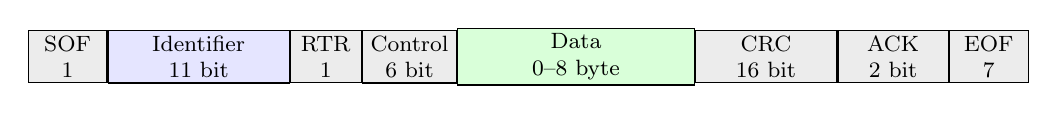
\begin{tikzpicture}[
  every node/.style={draw,minimum height=1.3em,font=\footnotesize,
    inner sep=2pt, align=center}]
\node[fill=gray!15,minimum width=1.0cm] (sof) {SOF\\1};
\node[right=0pt of sof,fill=blue!10,minimum width=2.3cm]  (id)  {Identifier\\11 bit};
\node[right=0pt of id,fill=gray!15,minimum width=0.9cm] (rtr) {RTR\\1};
\node[right=0pt of rtr,fill=gray!15,minimum width=1.2cm] (ctrl){Control\\6 bit};
\node[right=0pt of ctrl,fill=green!15,minimum width=3.0cm](data){Data\\0--8 byte};
\node[right=0pt of data,fill=gray!15,minimum width=1.8cm] (crc) {CRC\\16 bit};
\node[right=0pt of crc,fill=gray!15,minimum width=1.4cm] (ack) {ACK\\2 bit};
\node[right=0pt of ack,fill=gray!15,minimum width=1.0cm] (eof) {EOF\\7};
\end{tikzpicture}
\caption{Simplified layout of a classical CAN 2.0A data frame. The identifier field is used for bitwise arbitration; the data field carries the payload the application layer is interested in.}
\label{fig:can_frame}
\end{figure}

To prevent the transmitter and receivers from losing bit synchronisation during long runs of identical bits, CAN applies \textit{bit stuffing}: after five consecutive bits of the same polarity the transmitter inserts one bit of the opposite polarity, which the receivers remove again. This mechanism, together with the CRC and the acknowledgement slot, is part of the extensive error-handling machinery that gives CAN its characteristic robustness. The distinction between the 11-bit standard identifier (CAN~2.0A) and the 29-bit extended identifier (CAN~2.0B) is important for this thesis: ordinary broadcast traffic and many gateway ECUs use the shorter 11-bit form, whereas the addressed diagnostic exchange with the battery ECU relies on 29-bit extended identifiers, as detailed in Section~\ref{ssec:diag_addr}.

\subsection{Arbitration and Prioritisation}
CAN uses Carrier-Sense Multiple Access with Collision Resolution (CSMA/CR). When two or more nodes start transmitting simultaneously, each node reads back the bus level during its own transmission. Because a dominant bit (0) always wins over a recessive bit (1), the node with the numerically lower identifier automatically continues to transmit while the others switch to the listen state. The essential feature is that this collision resolution is \emph{non-destructive}: unlike Ethernet's classical CSMA/CD, where a collision destroys all colliding frames and forces a random back-off, CAN loses no information at all, because the winning message continues on the bus without interruption while the losing nodes seamlessly become receivers of that very message. This guarantees that the highest-priority message is never delayed by a collision.

A concrete walk-through makes the mechanism tangible. Suppose two nodes contend for the bus at the same time, one wishing to send identifier \canid{100} and the other \canid{101}. After the shared start-of-frame bit, both nodes begin to clock out their 11-bit identifiers most-significant-bit first, and because the leading bits of \hex{100} and \hex{101} are identical, both keep transmitting and both keep reading the bus without any disagreement. The two identifiers differ only in their least-significant bit: the first node drives a dominant 0 there, while the second drives a recessive 1. At that bit time the bus therefore settles to the dominant level. The second node, reading back the bus, sees a dominant 0 where it transmitted a recessive 1, recognises that it has lost arbitration, and immediately stops transmitting to become a receiver. The first node, whose transmitted bit matches the bus, notices nothing unusual and simply carries on sending the rest of its frame. No time is lost, no frame is corrupted, and the lower-numbered identifier has silently won. In an electric vehicle, safety-critical messages (such as the motor torque request or the battery current measurement) are therefore assigned low arbitration IDs, while convenience signals use higher IDs.

\subsection{Classical CAN vs.\ CAN-FD}
Two variants of the protocol are relevant. \textit{Classical CAN} (CAN~2.0, ISO~11898-1:2003) is limited to 8~payload bytes per frame and a single bit rate for the whole frame. \textit{CAN-FD} (CAN with Flexible Data-rate, standardised in ISO~11898-1:2015) extends this in two ways: the payload grows to up to 64~bytes, and the data phase of the frame may be transmitted at a higher bit rate than the arbitration phase, while the arbitration mechanism itself is unchanged. The motivation for CAN-FD was the growing bandwidth demand of modern vehicles: larger payloads reduce the protocol overhead per useful byte, and switching to a faster bit rate during the data phase -- once arbitration has already selected a single transmitter and the bit-wise, propagation-limited contention is over -- shortens the time the bus is occupied by each message. Crucially, because the arbitration phase is untouched, CAN-FD preserves the deterministic, priority-based bus access that makes Classical CAN attractive in the first place.

The diagnostic CAN bus exposed on the OBD-II connector of the ID.~Buzz operates as a \textbf{Classical CAN bus at 500~kbit/s with 11-bit broadcast identifiers}; the diagnostic exchange with the battery ECU additionally uses 29-bit extended identifiers (Section~\ref{ssec:diag_addr}). It is \emph{not} CAN-FD. This is the decisive constraint behind the methodology of this thesis: because each frame carries at most 8~bytes, every UDS response longer than 7~payload bytes must be segmented by ISO-TP, and a logger that can only emit single CAN frames cannot read those multi-frame identifiers (Section~\ref{sec:uds_procedure}). The data logger used here (CANedge2)~\cite{csselectronics_canedge2} electrically supports both Classical CAN and CAN-FD, but is configured for Classical CAN at 500~kbit/s to match the vehicle, with the CAN-FD data bit rate left defined (2~Mbit/s) only so that the controller can initialise. This single-frame limitation is not a peripheral detail but the central reason why some multi-byte identifiers can only be partially recovered in this work, and it motivates the deliberately selective, single-frame UDS strategy developed in the following chapters.

\section{Diagnostics: OBD-II, ISO-TP and UDS}
While the CAN bus is the low-level transport medium, automotive diagnostics rely on two additional layers built on top of CAN: a transport protocol that allows messages longer than 8~bytes to be fragmented and reassembled (ISO-TP), and an application layer that defines services, sub-functions and data identifiers (UDS). Both are accessed from outside the vehicle via a standardised connector: the OBD-II port. Together these three elements form a clean division of labour, in which each layer solves exactly one problem and hides its internal complexity from the layer above -- the physical connector standardises access, the transport layer standardises segmentation, and the application layer standardises the meaning of the exchanged data.

It is useful to locate each of these protocols in the OSI reference model before going into detail, because the rest of the thesis repeatedly refers to ``which layer'' a given problem belongs to. The diagnostic stack used here maps onto the OSI layers as summarised in Table~\ref{tab:osi_stack}: CAN occupies the two lowest layers, ISO-TP provides the network/transport function that classical CAN itself lacks, and UDS is the application protocol that the battery management ECU actually speaks. Thinking in terms of layers is not merely pedagogical bookkeeping: the single-frame limitation discussed above is a transport-layer problem, whereas the interpretation of an unknown data identifier is an application-layer problem, and keeping the two separate is what allows the methodology to reason precisely about where a given difficulty originates.

\begin{table}[H]
\caption{Mapping of the diagnostic protocol stack used in this thesis onto the OSI reference model.}
\label{tab:osi_stack}
\centering
\begin{tabular}{clp{6.6cm}}
\toprule
\textbf{OSI layer} & \textbf{Protocol} & \textbf{Role in this work} \\
\midrule
7 -- Application & UDS (ISO 14229)        & Services, sub-functions and Data Identifiers; \hex{22} \textit{ReadDataByIdentifier} returns the battery parameters. \\
6/5             & (not used)              & No presentation/session layer in CAN diagnostics. \\
4/3 -- Transport/Network & ISO-TP (ISO 15765-2) & Segments UDS messages longer than 7~bytes into First/Consecutive frames and reassembles them. \\
2 -- Data link  & CAN (ISO 11898-1)       & Frame format, arbitration, CRC, acknowledgement. \\
1 -- Physical   & CAN (ISO 11898-2)       & Differential CAN-H/CAN-L pair, 500~kbit/s, 120~$\Omega$ termination. \\
\bottomrule
\end{tabular}
\end{table}

\subsection{The OBD-II Connector (SAE J1962)}
All passenger cars sold in the European Union since 2004 (diesel: 2006) must expose a 16-pin diagnostic connector in the driver's footwell area, standardised by SAE J1962~\cite{saej1962}. The connector was originally mandated to make emission-related diagnostics uniformly accessible across manufacturers, so that a standard scan tool could read fault codes and emission parameters from any compliant vehicle without proprietary hardware. Two pins carry the high-speed CAN bus used for emissions diagnostics (pin~6 = CAN-H, pin~14 = CAN-L). On many manufacturers' vehicles, additional pins are used by a \textit{gateway ECU} that multiplexes private manufacturer buses onto the OBD-II connector only for authenticated diagnostic tester sessions. This gateway is central to the present work: it is precisely because the gateway does not forward the raw internal battery broadcast traffic to the OBD-II connector that a passive recording at the port cannot see the battery frames directly, and it is precisely because the gateway \emph{does} route addressed diagnostic requests inward to the battery ECU that an active query can still reach the data.

The physical interface is also what powers the measurement setup used later in this thesis. Beyond the two CAN pins, the connector provides a permanent supply and ground that allow a self-contained logger to draw its operating current directly from the vehicle without any separate power source. The pins relevant to this work are summarised in Table~\ref{tab:obd2_pins}.

\begin{table}[H]
\caption{Key pins of the SAE~J1962 OBD-II connector used in this thesis.}
\label{tab:obd2_pins}
\centering
\begin{tabular}{llp{7cm}}
\toprule
\textbf{Pin} & \textbf{Signal} & \textbf{Function} \\
\midrule
4  & Chassis ground           & Vehicle chassis reference. \\
5  & Signal ground            & Signal return. \\
6  & CAN-H (HS-CAN)           & High-speed CAN 500~kbit/s, used for OBD-II and UDS. \\
14 & CAN-L (HS-CAN)           & Complementary line to pin~6. \\
16 & Battery positive         & Permanent +12~V from the vehicle battery (used by the data logger). \\
\bottomrule
\end{tabular}
\end{table}

\subsection{ISO 15765-2 Transport Protocol}
A single classical CAN frame can carry only up to 8~bytes. UDS responses for an identifier such as ``read VIN'' or ``read DID'' routinely need more than 8~bytes. The ISO 15765-2 transport protocol~\cite{iso15765} solves this by fragmenting the application-layer PDU into multiple CAN frames of four possible types: \textit{Single Frame} (SF) for up to 7 bytes of payload, \textit{First Frame} (FF) plus a sequence of \textit{Consecutive Frames} (CF) for longer messages, and \textit{Flow Control} (FC) frames for sender throttling. The first byte (or first nibble) of each ISO-TP frame is a protocol-control-information (PCI) field that encodes the frame type and, depending on the type, either the total message length or the sequence number of the fragment, so that the receiver can distinguish the four cases and reassemble the fragments in the correct order.

\begin{figure}[H]
\centering
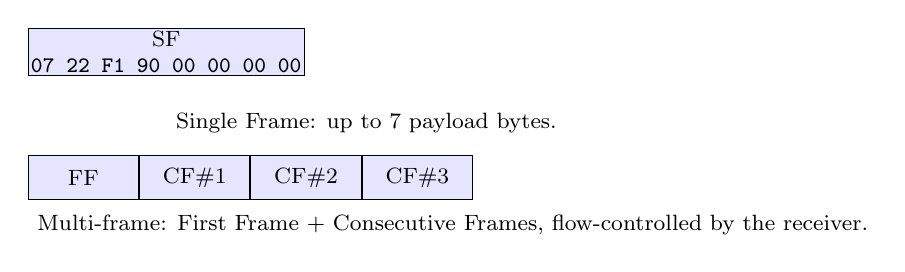
\begin{tikzpicture}[
  every node/.style={font=\footnotesize},
  tx/.style={draw,fill=blue!10,minimum height=1.6em,minimum width=1.4cm,inner sep=1pt,align=center},
  label distance=2pt]
\node[tx] (sf) {SF\\\texttt{07 22 F1 90 00 00 00 00}};
\node[below=0.6cm of sf,anchor=west] {Single Frame: up to 7 payload bytes.};

\node[tx,below=1.6cm of sf.west,anchor=west,minimum width=1.4cm] (ff) {FF};
\node[tx,right=0pt of ff,minimum width=1.4cm] (cf1){CF\#1};
\node[tx,right=0pt of cf1,minimum width=1.4cm] (cf2){CF\#2};
\node[tx,right=0pt of cf2,minimum width=1.4cm] (cf3){CF\#3};
\node[below=0.6cm of ff.west,anchor=west] {Multi-frame: First Frame + Consecutive Frames, flow-controlled by the receiver.};
\end{tikzpicture}
\caption{ISO 15765-2 (ISO-TP) protocol data units. Short diagnostic messages fit in a Single Frame; longer responses use First Frame + Consecutive Frames with Flow Control.}
\label{fig:isotp}
\end{figure}

The temporal interplay of these frame types between the diagnostic client (tester) and the server (ECU) is shown in Figure~\ref{fig:isotp_seq}. The tester opens the exchange with a Single Frame request; the ECU answers with a First Frame, waits for the tester's Flow Control frame and then streams the Consecutive Frames, spaced by the minimum separation time \texttt{STmin} requested in the Flow Control frame. The Flow Control frame is what makes segmentation reliable across devices of different speed: it lets the receiver dictate both the block size, that is how many Consecutive Frames it will accept before it must be polled again, and the \texttt{STmin} gap that the sender must insert between successive frames so that a slower receiver is never overrun. This dialogue is only possible if the requesting device is itself capable of sending a Flow Control frame in response to a First Frame; a logger that can emit nothing but a single, periodically repeated request frame cannot complete the handshake, which is the direct reason why multi-frame identifiers are recovered only as their First Frame in this work.

\begin{figure}[H]
\centering
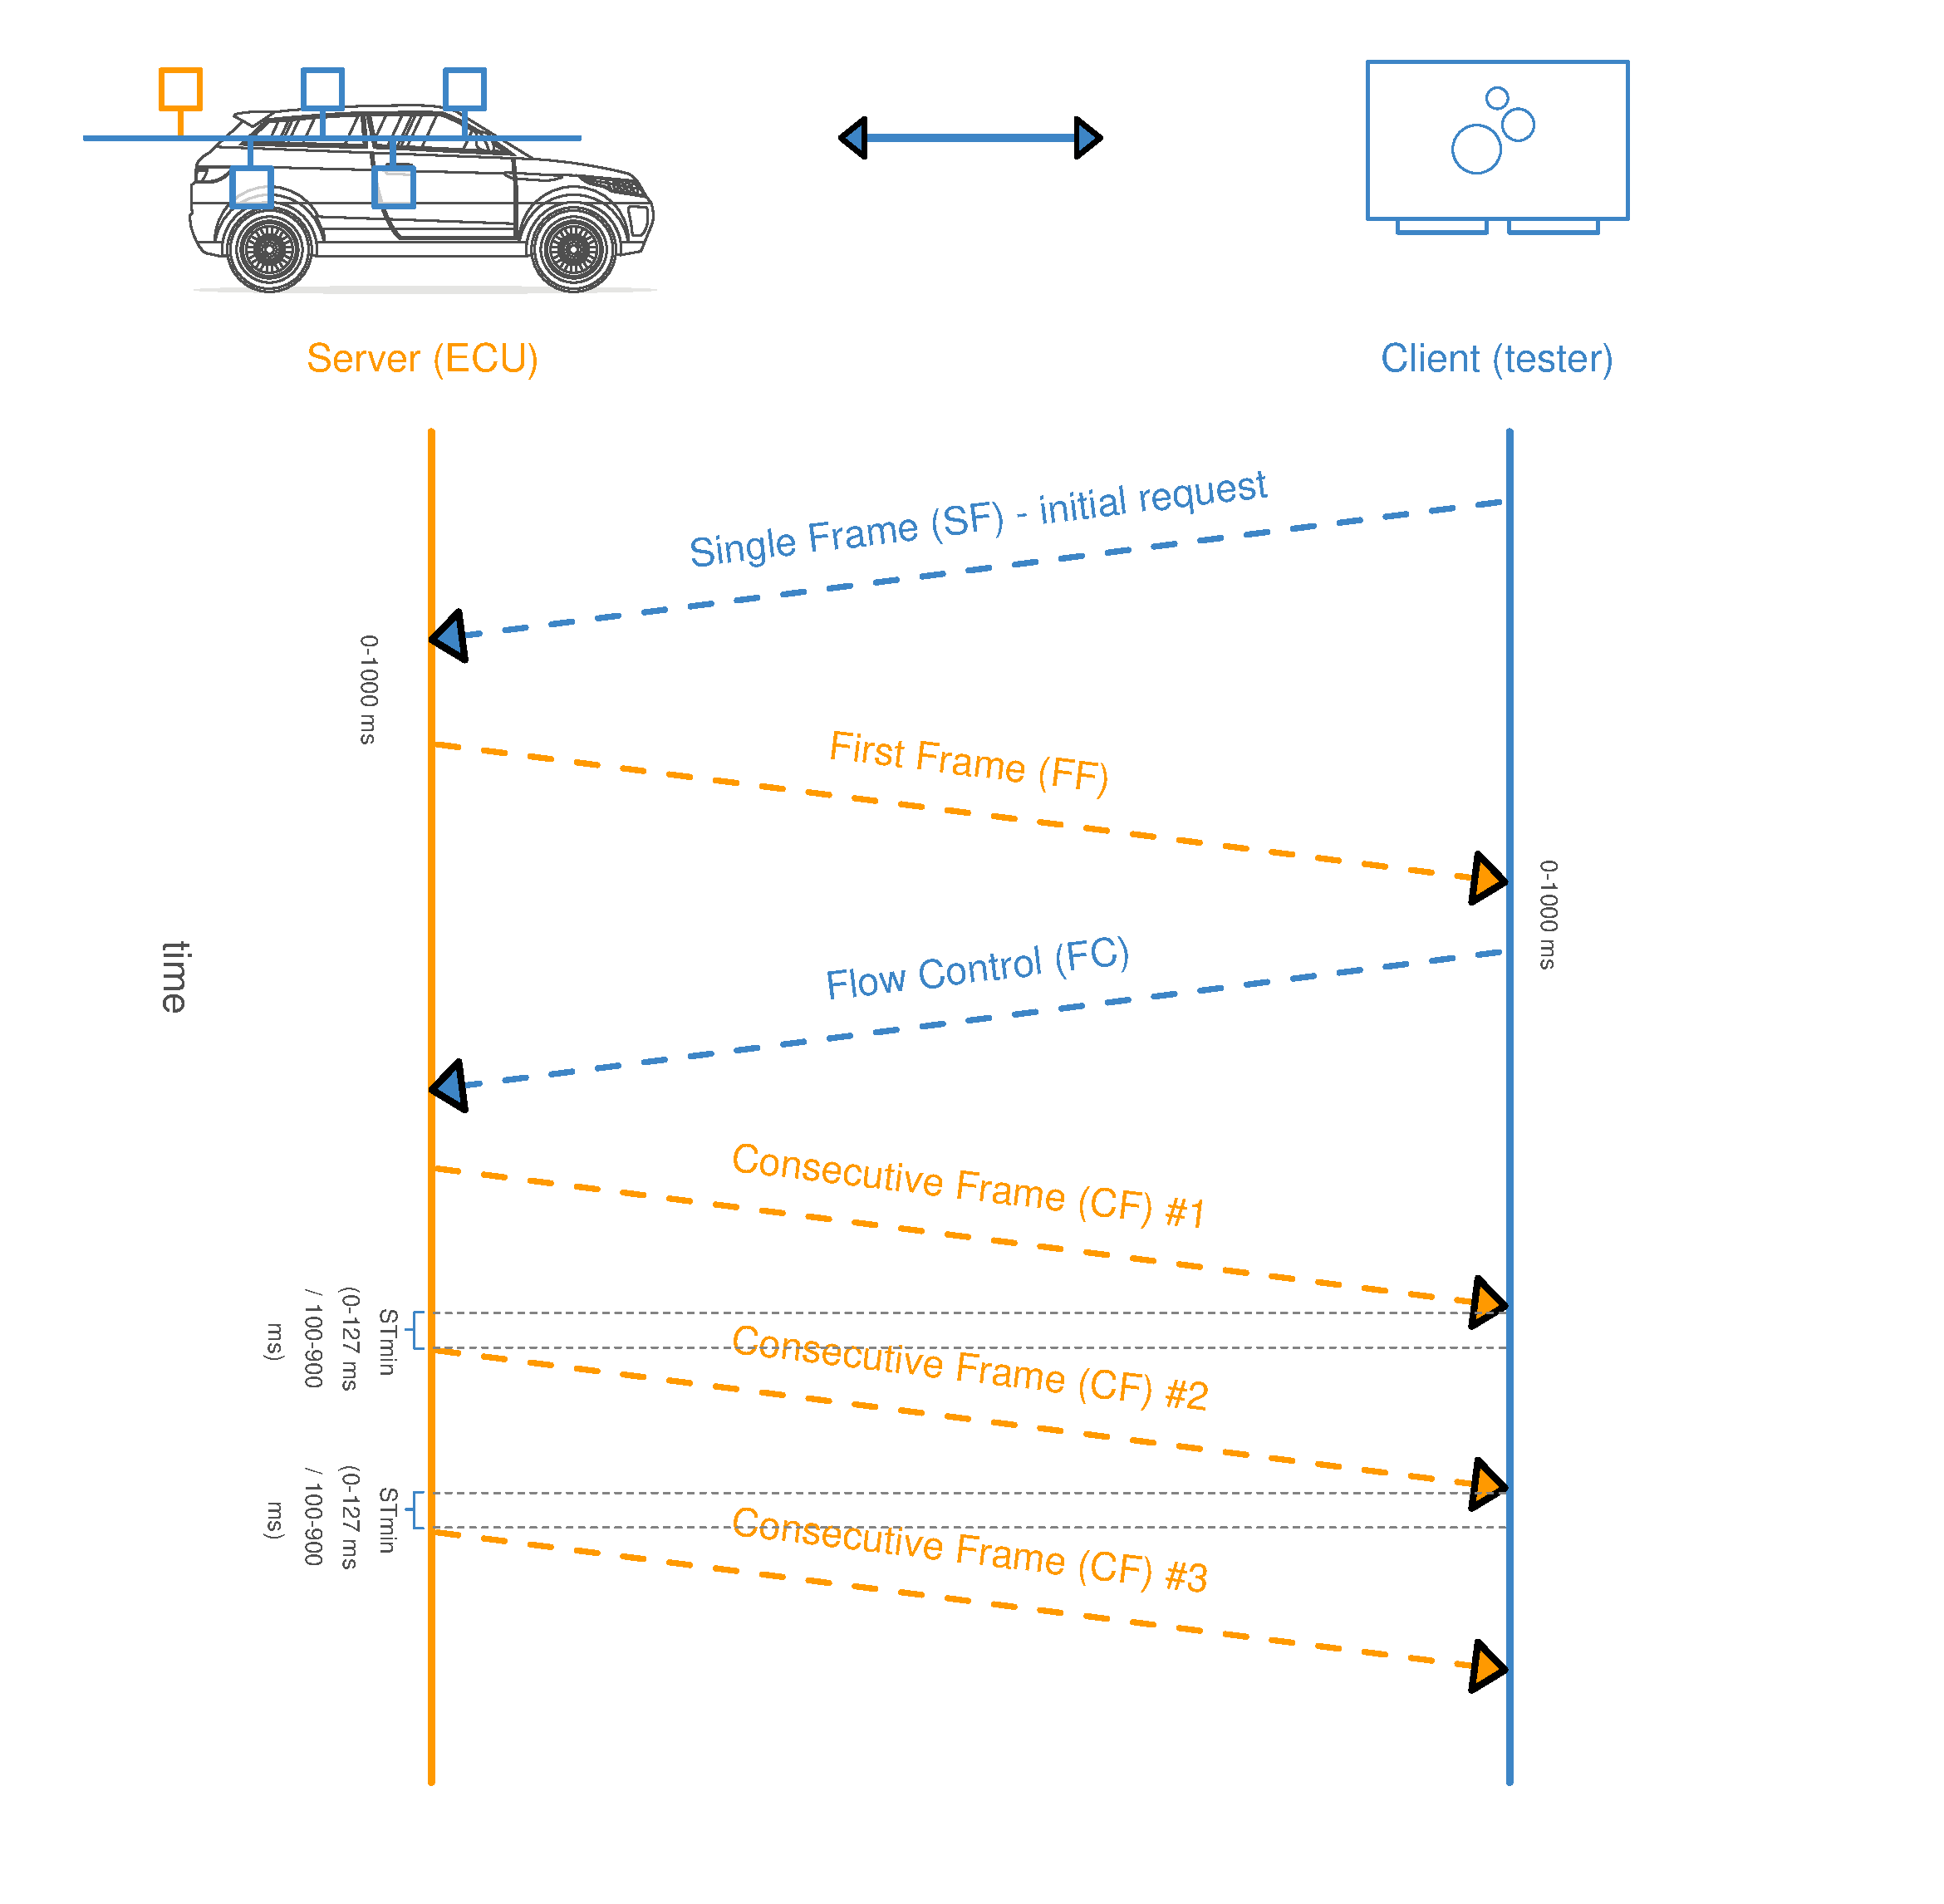
\includegraphics[width=0.78\textwidth]{implementation_uds_protocol.pdf}
\caption{ISO-TP message sequence between the tester (client) and the ECU (server) for a multi-frame UDS response: Single Frame request, First Frame, Flow Control, and Consecutive Frames separated by \texttt{STmin}.}
\label{fig:isotp_seq}
\end{figure}

\subsection{Unified Diagnostic Services (UDS)}
UDS, standardised in ISO 14229~\cite{iso14229}, is the \textbf{application-layer (OSI layer~7)} protocol used for all modern vehicle diagnostics, ECU programming and parameter reading. It sits at the very top of the diagnostic stack of Table~\ref{tab:osi_stack}: it defines \emph{what} is requested (services, sub-functions, Data Identifiers), while it deliberately says nothing about \emph{how} the bytes reach the ECU. The segmentation of long messages is delegated to ISO-TP one layer below (transport/network), and the actual bit transport to CAN at the data-link and physical layers. The same UDS service set therefore runs unchanged over CAN, CAN-FD, FlexRay, K-Line or DoIP/Ethernet -- only the lower layers differ. This layering is what makes UDS knowledge transferable: a service learned on one transport applies directly to any other, and the reverse-engineering strategy developed here would carry over to a future DoIP-based vehicle with the transport layer swapped out but the application dialogue intact.

Each UDS request is a byte stream starting with a one-byte Service Identifier (SID). The response either re-uses the SID increased by \hex{40} (positive response) or uses \hex{7F} followed by the original SID and an NRC (negative response code). For example, a read request with SID~\hex{22} is answered positively with SID~\hex{62}, or negatively with \hex{7F 22 \textit{NRC}} -- where the NRC \hex{31} means \textit{requestOutOfRange} (unknown DID/ECU) and \hex{33} means \textit{securityAccessDenied}. The negative response codes are informative in their own right during reverse engineering: a \hex{31} response tells the tester that the queried identifier is not implemented on that ECU and can be pruned from the search, whereas a \hex{33} response reveals that the identifier exists but lies behind a security-access barrier and would require a seed/key exchange to read. Distinguishing these two failure modes is what turns a blind sweep of candidate identifiers into a systematic mapping of what a given ECU exposes.

The services most relevant to this thesis are summarised in Table~\ref{tab:uds_services}. In particular, service \udssid{22} (\textit{ReadDataByIdentifier}) allows a tester to request the value of a specific two-byte Data Identifier (DID). Manufacturer-specific DIDs in the range \hex{F100}--\hex{FFFF} are routinely used by Volkswagen to expose battery parameters. Before such reads succeed, however, the tester usually has to raise the ECU out of its default session with \hex{10} (\textit{DiagnosticSessionControl}) into an extended session, and then keep that session alive with periodic \hex{3E} (\textit{TesterPresent}) messages, since an idle session times out and falls back to default after a few seconds. The interplay of these three services -- open the session, keep it alive, read the identifier -- forms the backbone of the acquisition procedure described in Section~\ref{sec:uds_procedure}.

\begin{table}[H]
\caption{UDS services relevant to the retrieval of battery data.}
\label{tab:uds_services}
\centering
\begin{tabular}{clp{7cm}}
\toprule
\textbf{SID} & \textbf{Service}             & \textbf{Purpose} \\
\midrule
\hex{10}     & DiagnosticSessionControl    & Switch between default, programming or extended session. \\
\hex{22}     & ReadDataByIdentifier        & Read the value stored under a 16-bit DID. \\
\hex{27}     & SecurityAccess              & Unlock protected data ranges via seed/key. \\
\hex{2E}     & WriteDataByIdentifier       & Write a value under a DID (not used here). \\
\hex{3E}     & TesterPresent               & Keep an extended session alive. \\
\bottomrule
\end{tabular}
\end{table}

\subsection{Diagnostic Addressing for Battery Data}
\label{ssec:diag_addr}
For a VW~Group vehicle built on the MEB platform, the battery management ECU (``HV battery'', BMS) answers on its own diagnostic CAN ID pair using 29-bit extended addressing. On the ID.~Buzz examined here the BMS is reached with request ID \hex{17FC007B} and replies on \hex{17FE007B}. This request/reply pairing is an instance of \emph{physical} (point-to-point) addressing: a request is directed at exactly one ECU, which answers on a fixed, closely related reply identifier, so that the tester can associate each response unambiguously with the ECU it queried. Other ECUs follow the same \hex{17FC00xx}/\hex{17FE00xx} scheme (e.g.\ DC/DC converter \hex{17FC00B9}/\hex{17FE00B9}, front EDU \hex{17FC0076}/\hex{17FE0076}), while a few comfort/gateway ECUs answer on classic 11-bit pairs (e.g.\ climate \hex{746}/\hex{7B0}, gateway \hex{710}/\hex{77A}). The regularity of the extended-identifier scheme, in which the low byte selects the target ECU, is itself a useful piece of reverse-engineering knowledge, because it lets a newly discovered ECU be addressed by analogy once the pattern is known.

A functional request to \hex{7DF} (the OBD-II broadcast request ID) reaches all emission-relevant ECUs simultaneously and is the starting point for any tester that does not yet know the physical addressing. In contrast to physical addressing, this \emph{functional} form is a one-to-many broadcast: every ECU that implements the requested service may answer, so the tester can discover which ECUs are present and which services they support before committing to a specific physical address. In practice a diagnostic session therefore often begins functionally, to enumerate the responders, and then continues physically, to interrogate a chosen ECU -- here the battery management controller -- in detail.

\section{The Volkswagen MEB Platform}
The Modular Electric Drive Matrix (\textit{Modularer E-Antriebs-Baukasten}, MEB) is Volkswagen Group's dedicated BEV platform, first used in production on the ID.3 in 2019. Unlike earlier electric vehicles that were adapted from combustion-engine platforms, the MEB was designed from the ground up around the battery and electric drivetrain, which allows a more efficient use of space and a network architecture tailored to the needs of an electric vehicle rather than retrofitted onto a legacy design. All ID-series vehicles -- including the ID.~Buzz used in this thesis -- share the same underlying architecture: a modular skateboard chassis with a flat battery pack between the axles, a rear-mounted permanent-magnet synchronous motor (single-motor variants) or an additional asynchronous motor on the front axle (4Motion variants), and a fully redesigned in-vehicle electrical and electronic architecture. Because the platform is shared across the whole ID family, insight gained on one MEB vehicle -- including the diagnostic addressing and the identifier layouts studied here -- is expected to transfer, at least in part, to its siblings.

From an electronic networking point of view, the MEB is organised around a small number of domain controllers (drive, chassis, comfort, infotainment, charging) connected to a central gateway ECU. Grouping functions into domains reduces the number of buses that must be interconnected and concentrates cross-domain routing in a single, well-defined place. The gateway isolates the private manufacturer CAN buses from the OBD-II connector; external testers see either the OBD-II emission CAN bus directly or -- in extended diagnostic sessions -- a subset of the internal buses routed through the gateway by UDS. This isolation is a deliberate design choice with both a safety and a security rationale: it prevents an external device from injecting arbitrary traffic onto the powertrain and battery buses, and it hides the internal broadcast messages -- including the raw battery frames -- from anything plugged into the diagnostic port. It is exactly this property that rules out a purely passive, byte-level recording of the battery traffic at the OBD-II connector and that makes the active, UDS-based approach of this thesis necessary.

The traction battery of the ID.~Buzz (Pro variant) has a gross capacity of 82~kWh (77~kWh net) at a nominal pack voltage of around 400~V. It is managed by a dedicated Battery Management Controller (BMC) and a series of cell-supervision circuits (CSC) that continuously report cell voltages and temperatures to the BMC over an internal battery CAN. This internal battery CAN is one of the private buses that the gateway keeps separate from the diagnostic port, so the detailed cell data it carries is not visible from the outside as ordinary broadcast traffic; it becomes reachable only when the BMC is addressed directly through the diagnostic services described above.

\section{High-Voltage Battery Systems in BEVs}
The lithium-ion pack of a modern BEV is not simply a larger version of a 12~V starter battery. It is an active system composed of several hundred individual cells, grouped into modules, managed by a dedicated electronic hierarchy. Where a starter battery is a passive energy store that is charged and discharged within a narrow band and largely ignored by the rest of the vehicle, a traction pack must be continuously supervised at the level of the individual cell, because both the safety and the usable lifetime of the pack depend on keeping every cell within tight voltage and temperature limits. The remainder of this section introduces the physical structure of the pack, the duties of the electronics that manage it, and the specific quantities this thesis sets out to observe.

\subsection{Cell, Module and Pack}
A single Li-ion cell has a nominal voltage of 3.6--3.7~V. In the ID.~Buzz, cells are connected in series to reach the pack nominal voltage, and in parallel to reach the desired capacity. The cells are organised into modules; each module has its own cell-supervision circuit that measures individual cell voltages (one measurement per cell) and one or more module temperatures. This three-level hierarchy -- cell, module, pack -- is what allows the management electronics to reason about the pack at the right granularity: safety decisions such as opening the contactors depend on the extreme values across all cells, whereas balancing and diagnostics depend on the value of each cell individually. Because the series connection means the weakest cell limits the whole string, per-cell measurement is not a luxury but a requirement, and it is the reason the pack exposes a long list of individual cell-voltage identifiers rather than a single aggregate figure.

\subsection{Battery Management System}
The Battery Management System (BMS) is responsible for keeping the pack within its safe operating area. It continuously compares the measured cell voltages, temperatures and currents against the limits defined for the chemistry, and it intervenes -- by limiting power, requesting cooling or heating, or ultimately opening the contactors -- whenever a limit is approached, so that the pack is protected against overcharge, deep discharge, over-current and thermal runaway. Its core duties are:

\begin{itemize}
  \item monitoring every cell voltage and every module temperature;
  \item estimating the pack state of charge (SOC) and state of health (SOH);
  \item controlling the main positive and negative contactors;
  \item performing cell balancing (passive or active) during charging;
  \item reporting power limits (charge/discharge) to the inverter and the charger.
\end{itemize}

Each of these duties leaves an observable trace in the data the BMS holds internally, and it is this internal state that the diagnostic queries of this thesis aim to read out. The monitoring duty produces the per-cell voltage and per-point temperature values; the estimation duty produces the SOC and SOH figures shown on the dashboard; the contactor and power-limit duties determine the operating mode the pack reports. Reconstructing the meaning of the corresponding data identifiers is therefore, in effect, reconstructing a view of the BMS's own working picture of the pack.

SOC in particular is not a directly measurable quantity. It is estimated by the BMS from a combination of coulomb counting, open-circuit-voltage look-ups and model-based filters such as Kalman filters. Coulomb counting integrates the measured current over time to track how much charge has entered or left the pack, but it accumulates drift and must be periodically corrected; the open-circuit voltage of a cell at rest gives an independent, if slow, anchor for the true state of charge; and a model-based filter fuses these sources while accounting for their respective uncertainties. The estimate that the BMS reports to the driver's dashboard is therefore a conservative, smoothed version of a much richer internal state. This indirection matters for the validation strategy of this thesis: because the reported SOC is a filtered estimate rather than a raw sensor reading, agreement between a decoded identifier and the dashboard value confirms not only that the byte layout and scaling are correct but also that the identifier being read is indeed the one the BMS presents to the driver.

\subsection{Signals of Interest}
For this thesis, the following battery parameters are considered the primary targets. They were chosen because together they span the safety-critical and the informational aspects of the pack: the aggregate quantities (state of charge, terminal voltage, current, state of health) describe the pack as a whole, while the per-cell extremes (minimum and maximum cell voltage and temperature) describe its internal spread and therefore its health and safety margin. Recovering these quantities, and confirming their scaling against the physical vehicle, is the concrete objective around which the acquisition and decoding chapters are built.

\begin{table}[H]
\caption{Battery parameters targeted by the UDS queries in this thesis.}
\label{tab:battery_signals}
\centering
\begin{tabular}{lp{4cm}l}
\toprule
\textbf{Parameter}           & \textbf{Typical scale}             & \textbf{Expected DID range} \\
\midrule
Pack state of charge         & 0--100\,\%, 0.5\,\% resolution     & manufacturer-specific \\
Pack terminal voltage        & 0--500\,V, 0.1\,V resolution       & manufacturer-specific \\
Pack current                 & $\pm$500\,A, signed, 0.1\,A res.   & manufacturer-specific \\
Cell voltage min / max       & 2.5--4.25\,V, 1\,mV resolution     & manufacturer-specific \\
Cell temperature min / max   & $-40$\,\textdegree{}C--+80\,\textdegree{}C & manufacturer-specific \\
State of health              & 0--100\,\%                         & manufacturer-specific \\
\bottomrule
\end{tabular}
\end{table}

\section{State of the Art of CAN Bus Reverse Engineering}
The systematic reverse engineering of automotive CAN networks has been pursued in both the research and the open-source communities, motivated by the fact that the mapping from raw bus traffic to physical signals is almost never published by vehicle manufacturers. Two lines of prior work are directly relevant to the present thesis: the community-maintained effort to collect and share signal databases across many vehicles, and the vehicle-specific reverse engineering of high-voltage battery data.

On the open-source side, the \texttt{opendbc}~\cite{opendbc} repository maintained by comma.ai collects community-contributed CAN signal descriptions for a large number of vehicles. Such a shared database is valuable both as a source of candidate identifiers -- a starting point for what to look for on a related vehicle -- and as a means of cross-checking a newly reconstructed signal against what the community has already documented. In this thesis the community database plays exactly this supporting role: it provides an independent reference against which the manufacturer-specific data identifiers selected for extraction can be compared, so that the reverse-engineering effort does not begin from a blank slate but builds on and validates against existing community knowledge.

For electric vehicles in particular, Huybrechts et al.~\cite{huybrechts2018reverse} have demonstrated the reverse engineering of battery-related signals on a Tesla Model S, recovering physical battery quantities from otherwise undocumented traffic and validating them against the vehicle. Their work establishes both the feasibility and the general methodology of recovering meaningful battery parameters from an undocumented in-vehicle network, and it provides the closest point of comparison for the approach taken here. The present thesis differs chiefly in its vehicle and in the constraint imposed by the MEB gateway: because the raw battery frames are not exposed at the diagnostic port, the recovery relies on active UDS queries rather than passive observation, and the reconstructed identifiers are validated against the physical vehicle in the same spirit as this prior work.

% ============================================================

% ============================================================
\chapter{Materials and Methods}
% ============================================================
This chapter explains the selection of the test vehicle, the preparation of the measurement hardware, the experimental setup and the software tool chain used to record and analyse the CAN data. The order of presentation deliberately follows the physical signal path: from the vehicle that produces the battery data, through the logger that both stimulates and records the diagnostic bus, to the offline software that converts the raw log into engineering quantities. Each stage is described together with the reasoning behind the design choice, because several of these choices -- in particular the use of a transmit-capable logger and the decision to interrogate the battery actively rather than to observe it passively -- are direct consequences of how the vehicle architecture exposes (and, more importantly, hides) the battery-management data. The reverse-engineering methodology and the concrete diagnostic procedure that build on this setup are then developed in the later sections of the chapter.

\section{Test Vehicle: Volkswagen ID.~Buzz}
All measurements were performed on a 2024 Volkswagen ID.~Buzz Pro on loan to the CARISSMA research institute. The vehicle is representative of the MEB platform: 77~kWh net battery capacity, rear-wheel drive with a 150~kW permanent-magnet synchronous motor, and the current generation of Volkswagen's ID software (ID.~Software~4.x). Before every measurement session the vehicle was charged to approximately 90\,\% SOC at the CARISSMA AC wall-box in order to remove any low-SOC power derating from the results.

The choice of this particular vehicle is not incidental. The Modular Electric Drive Matrix (Modularer E-Antriebs-Baukasten, MEB) is Volkswagen's dedicated battery-electric platform and underpins a large family of production vehicles that share the same high-voltage architecture, the same battery-management electronics and the same diagnostic addressing scheme. Findings obtained on the ID.~Buzz therefore transfer, at least in their structure, to other MEB vehicles such as the ID.3 and ID.4, which is what makes the vehicle a useful and generalisable object of study rather than a one-off case. The 77~kWh net pack (82~kWh gross) operates at a nominal voltage of roughly 400~V and is assembled from 108 individual cells, a level of internal detail that becomes directly relevant once the reverse engineering descends to per-cell voltages and per-point temperatures. Because the ID.~Buzz is a recent, series-production vehicle running current ID.~Software, it also exhibits the full production security posture of the platform -- including the gateway isolation discussed in Section~\ref{sec:why_uds} -- so the constraints encountered here are the real constraints a workshop or researcher would face, not artefacts of a pre-series prototype.

Charging to approximately 90\,\% SOC before each session serves a specific experimental purpose. At low states of charge the battery-management system progressively limits available power and alters the operating point of the pack, which would confound any attempt to compare decoded values against a stable physical reference. Starting each session from a high, well-defined SOC keeps the pack in a comfortable operating band, so that the quantities read back over the diagnostic bus reflect the normal working state of the battery rather than a derated corner case. This matters for the validation step of the methodology, where each decoded value is checked against the externally observable state of the vehicle: a stable and representative operating point makes those comparisons meaningful.

\section{Hardware Setup}
\subsection{CANedge2 Data Logger}
The CAN frames were recorded with a CANedge2 data logger (CSS Electronics)~\cite{csselectronics_canedge2}. This device has two independent CAN channels, each with a 24-bit hardware timestamp, supports CAN Classical and CAN-FD, and stores data on an SD card in the ASAM~MDF~4.11 format~\cite{asammdf}. Its power is drawn from pin~16 (battery~+) of the OBD-II connector, which means the logger stays active as long as the vehicle has power -- including the short wake-up interval after the vehicle is unlocked. Channel~1 was configured for Classical CAN at 500~kbit/s; channel~2 was left in listen-only mode for an optional second tap.

The hardware timestamp deserves emphasis, because the entire later analysis relies on being able to associate each response with the request that provoked it. A 24-bit timestamp generated in the logger's own hardware, rather than assigned in software after the fact, means that every frame -- transmitted or received -- carries a precise and monotonic time reference from a single clock. When requests and responses are written into the same file with the same time base, matching a positive UDS answer to its originating ReadDataByIdentifier request becomes a straightforward temporal-proximity problem instead of a fragile reconstruction. The 500~kbit/s Classical CAN configuration on channel~1 matches the physical characteristics of the OBD-II diagnostic bus of the ID.~Buzz, which is a Classical CAN bus and not CAN-FD~\cite{iso11898}; configuring the channel to the exact bus bit rate is a precondition for the controller to acknowledge frames and participate on the bus at all. Channel~2 was held in listen-only mode as an optional second tap, so that an additional bus could be observed without any risk of the logger disturbing it.

\begin{figure}[H]
\centering
\begin{subfigure}[b]{0.48\textwidth}
  \centering
  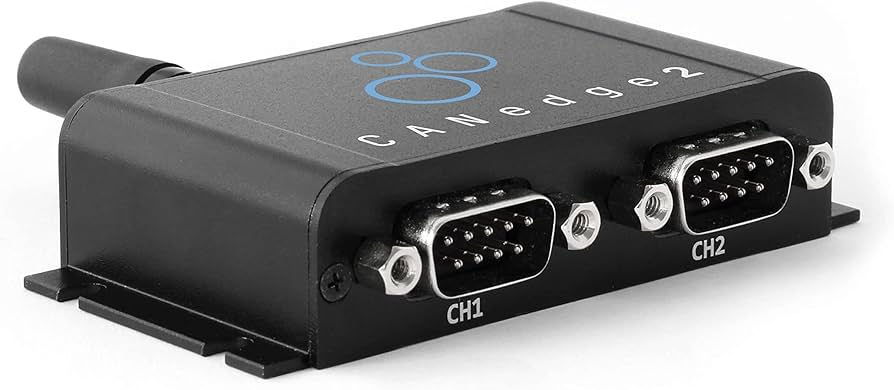
\includegraphics[height=3.0cm]{front_view_canedge2_trim.png}
  \caption{Front view: the two DB9 connectors CH1 and CH2.}
  \label{fig:canedge_front}
\end{subfigure}
\hfill
\begin{subfigure}[b]{0.48\textwidth}
  \centering
  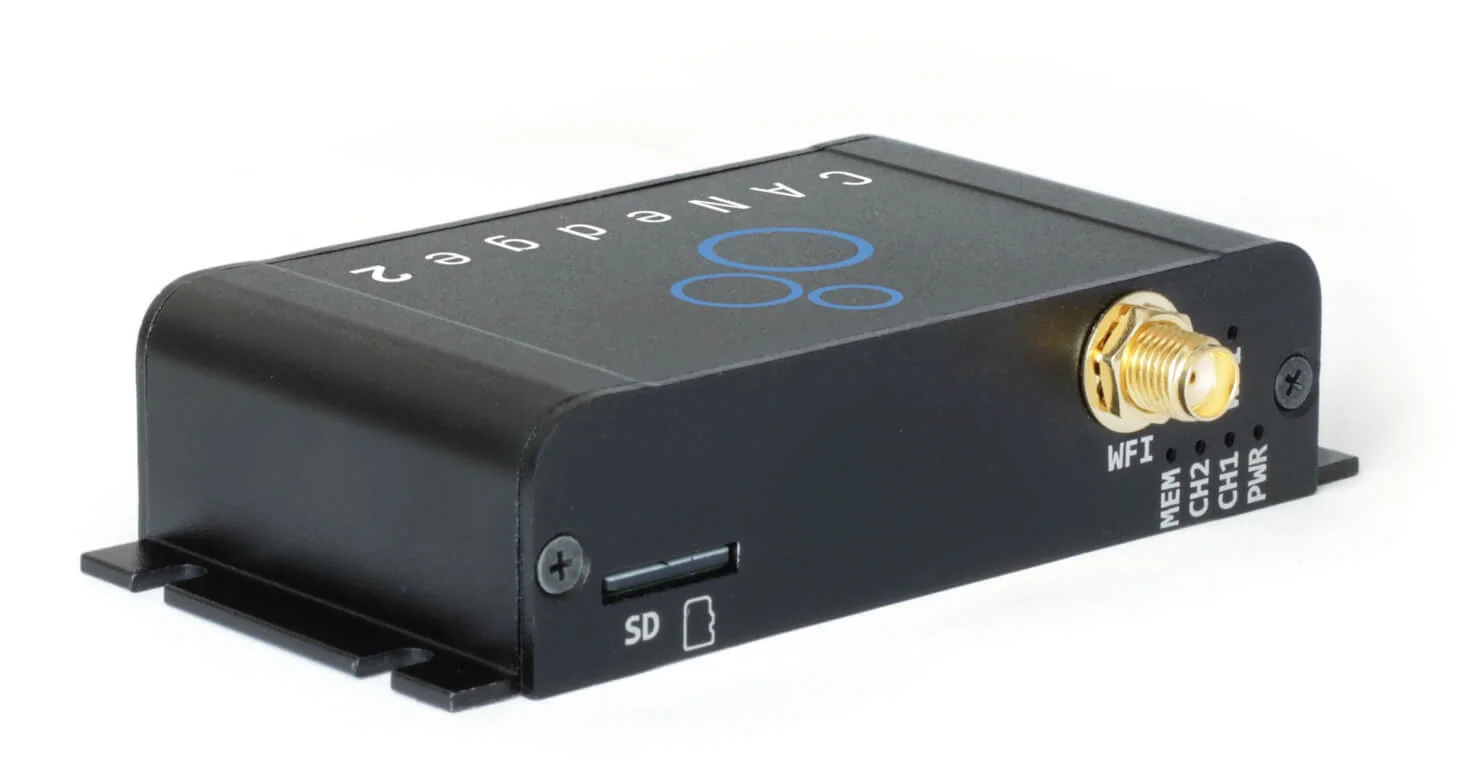
\includegraphics[height=3.0cm]{back_view_canedge2_trim.png}
  \caption{Rear view with the SD-card slot.}
  \label{fig:canedge_back}
\end{subfigure}
\caption{The CANedge2 data logger (CSS Electronics) used in this thesis. CH1 is connected to the OBD-II HS-CAN bus of the ID.~Buzz; CH2 is left in listen-only mode.}
\label{fig:canedge2}
\end{figure}

Crucially, the CANedge2 is not only a passive logger: each CAN channel has a configurable \textit{transmit list} that can periodically send up to 64 user-defined CAN frames onto the bus and log the responses in the same MF4 file. In this thesis that transmit list is used to issue the UDS requests directly from the logger, so that \textbf{the active UDS retrieval of battery data is performed by the CANedge2 itself} rather than by a separate diagnostic tester. This makes the active and passive data appear in one synchronised, hardware-timestamped recording. The device used here runs firmware~01.08.01 with configuration schema~01.08.

The transmit capability is the single most important reason the CANedge2 was chosen over a purely passive logger, because the battery data on this platform cannot be recovered by listening alone (Section~\ref{sec:why_uds}); it must be elicited by sending diagnostic requests. A conventional logger would force the setup to include a second, separately clocked device -- a dedicated diagnostic tester -- to generate those requests, after which the requests and the responses would live in two files with two time bases that must be aligned in post-processing. By collapsing the stimulus and the recording into one device, the transmit list eliminates that alignment problem entirely and guarantees that every logged response is timestamped on the same clock as the request that caused it. The consequence of this design choice, both its benefits and its one significant limitation, runs through the whole of the diagnostic procedure described in Section~\ref{sec:uds_procedure}.

\subsection{OBD-II Connection}
The CANedge2 was connected directly to the vehicle's OBD-II socket with a standard OBD-II--to--DB9 adapter cable on channel~1; no Y-splitter or parallel tester was used. The cable carries the CAN-H, CAN-L, ground and battery-positive lines on pins~6, 14, 4/5 and 16 respectively (compare Table~\ref{tab:obd2_pins}), so the logger is both powered and bus-connected through the single OBD-II connector.

The decision to use a single, direct connection rather than a Y-splitter feeding both the logger and a workshop tester in parallel is deliberate and has a clear technical justification. The OBD-II connector and its pin assignment are standardised~\cite{saej1962}, so a direct adapter reliably exposes the high-speed CAN pair together with ground and switched battery power on the pins listed above. Adding a second active device on the same bus through a splitter would introduce another node that arbitrates for the bus, acknowledges frames and potentially issues its own diagnostic traffic. On a diagnostic bus that traffic could collide or interleave with the requests emitted by the transmit list, could open or reset diagnostic sessions on the very ECUs under study, and would in any case make it impossible to attribute observed responses unambiguously to the logger's own requests. Keeping the CANedge2 as the sole diagnostic node on the bus removes these confounders, so that every request on the bus is one the logger sent and every response can be traced back to it. Drawing both power and bus connection through the single OBD-II connector also keeps the physical setup minimal and repeatable, which matters for a measurement that is rotated across several sessions and configurations.

\begin{figure}[H]
\centering
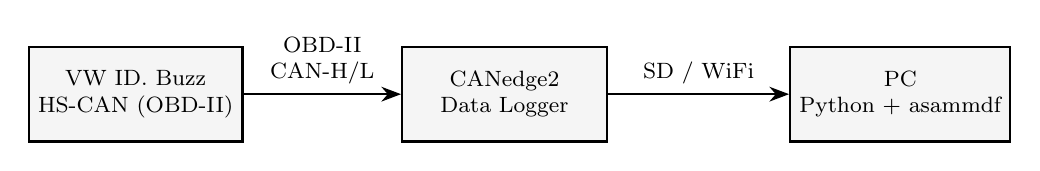
\begin{tikzpicture}[
  node distance=1.1cm and 1.4cm,
  every node/.style={font=\footnotesize},
  box/.style={draw,thick,minimum height=1.2cm,minimum width=2.6cm,align=center,fill=gray!8},
  bus/.style={draw,thick,-{Stealth[length=2.5mm]}}]

\node[box] (car) {VW ID.~Buzz\\HS-CAN (OBD-II)};
\node[box,right=2.0cm of car] (logger) {CANedge2\\Data Logger};
\node[box,right=2.3cm of logger] (pc) {PC\\Python + asammdf};

\draw[bus] (car) -- (logger) node[midway,above,align=center]{OBD-II\\CAN-H/L};
\draw[bus] (logger) -- (pc) node[midway,above]{SD / WiFi};
\end{tikzpicture}
\caption{Overall measurement setup. The CANedge2 logger is connected directly to the OBD-II connector of the vehicle, is powered from pin~16 of that connector, and writes MDF4 files to its SD card for offline analysis on the PC.}
\label{fig:setup}
\end{figure}

\section{Software Tool Chain}
The recorded MDF4 files were processed entirely in Python~3.13. The actual conversion from the binary MF4 log into engineering data is performed by the \textbf{\texttt{asammdf}} library~\cite{asammdf}: it parses the ASAM~MDF~4.11 container, decodes the embedded CAN frame groups (arbitration ID, DLC, raw payload bytes and hardware timestamp) and exposes them as \texttt{numpy} arrays. A thin custom module, \texttt{mf4\_reader.py} (built on \texttt{asammdf} together with \texttt{numpy} and \texttt{pandas}), flattens each frame into a \texttt{pandas} DataFrame with the columns described in Table~\ref{tab:mf4_columns}; a companion converter (\texttt{mf4\_converter.py}) uses the same \texttt{asammdf} backend to export the raw frames to SavvyCAN-compatible CSV for cross-checking. The physical battery quantities are then obtained by applying the per-DID scaling formulas of the master PID list (Section~\ref{sec:uds_procedure}) to the decoded UDS response bytes.

Building the tool chain on top of \texttt{asammdf} rather than parsing the binary container by hand is a pragmatic choice: the MF4 container is a rich, standardised format with channel groups, conversion rules and metadata, and a mature library handles the low-level container details reliably so that the analysis code can work with clean \texttt{numpy} arrays. Flattening each frame into a uniform DataFrame, as defined in Table~\ref{tab:mf4_columns}, gives every later stage of the pipeline a single, predictable data structure to operate on, independent of which log or which session a frame came from. The parallel export to SavvyCAN-compatible CSV via \texttt{mf4\_converter.py} provides an independent way to inspect the same raw frames in an established CAN-analysis tool, which is valuable as a cross-check during reverse engineering: if a frame is misread in the custom pipeline, the discrepancy against the SavvyCAN view surfaces it immediately.

\begin{table}[H]
\caption{Normalised frame format used across the analysis pipeline.}
\label{tab:mf4_columns}
\centering
\begin{tabular}{lll}
\toprule
\textbf{Column} & \textbf{Type}       & \textbf{Description} \\
\midrule
timestamp       & float (index)      & Seconds from recording start. \\
can\_id         & int                & 11-bit CAN arbitration ID. \\
can\_id\_hex    & string             & Hex representation, e.g.\ \texttt{0x065}. \\
dlc             & int                & Data-length code, 1--8. \\
data\_bytes     & byte array         & Raw payload. \\
data\_hex       & string             & Space-separated hex payload. \\
bus\_channel    & int                & CAN channel (fixed at 9). \\
direction       & int                & 0 = received. \\
source          & string             & Source log folder identifier. \\
\bottomrule
\end{tabular}
\end{table}

On top of \texttt{mf4\_reader.py} the analysis pipeline comprises:

\begin{itemize}
  \item \texttt{can\_analyzer.py} -- enumerates the CAN IDs present in a log and counts the request/response frames, used to verify that each UDS request received an answer.
  \item \texttt{uds\_decoder.py} -- extracts the UDS response frames that the CANedge2 logged on the BMS reply ID \hex{17FE007B}, matches each one to its request, and decodes the Data Identifier payloads into physical battery parameters using the per-DID scaling formulas.
\end{itemize}

These two modules separate two distinct concerns. The \texttt{can\_analyzer.py} module operates at the level of the bus itself: by enumerating the arbitration IDs present in a log and counting request and response frames, it answers the bookkeeping question of whether the diagnostic exchange actually completed -- that is, whether each request that was transmitted was in fact answered. The \texttt{uds\_decoder.py} module operates one layer higher, at the level of the diagnostic protocol: it isolates the UDS responses that the BMS returned on its reply identifier \hex{17FE007B}, pairs each response with the request that elicited it, and applies the per-DID scaling formulas to turn the raw payload bytes into physical battery parameters. This layered structure mirrors the reverse-engineering methodology of Section~\ref{sec:re_methodology}: coverage and completeness are established first, and only the responses that are actually present are then interpreted and scaled.

\section{Why Active UDS Instead of Passive Reverse Engineering}
\label{sec:why_uds}
Classical CAN reverse engineering is \textit{passive}: the analyst taps the bus on which the target ECU broadcasts, records its frames and recovers the signal layout statistically. This was the originally planned approach for the BMS of the ID.~Buzz, but it is not feasible from the OBD-II connector. The BMS broadcasts its raw measurement frames only on the private internal battery/powertrain CAN bus. On the MEB platform a central gateway ECU separates these internal buses from the OBD-II diagnostic bus and, for security reasons, does not forward the raw BMS broadcast frames to the outside. Consequently, the broadcast traffic visible on the OBD-II port does not contain the BMS measurement frames, and a passive byte-level reverse engineering of the battery signals cannot be performed without invasively tapping the high-voltage battery wiring -- which is out of scope and unsafe on a production vehicle.

The role of the gateway is central to understanding this constraint. In a modern vehicle the individual CAN buses are not one flat network; they are segmented into domains -- powertrain, chassis, comfort, infotainment and a dedicated diagnostic connection -- that are joined only through a central gateway ECU. The gateway acts as a controlled boundary: it decides which messages cross from one domain to another and which do not. The private battery and powertrain bus, on which the BMS continuously broadcasts its cyclic measurement frames, sits behind this boundary. From a security and robustness standpoint there is no reason for the manufacturer to relay those internal broadcast frames to the externally accessible OBD-II bus, and on the MEB platform they are not relayed. A passive tap on the OBD-II connector therefore sees the diagnostic traffic and whatever the gateway chooses to expose, but never the raw BMS broadcasts themselves. This is precisely the difference from earlier passive reverse-engineering studies on other manufacturers' vehicles, such as the recovery of battery data from the CAN bus of a Tesla Model~S~\cite{huybrechts2018reverse}, where the relevant frames were observable on an accessible bus; on the gated MEB architecture that observability is deliberately absent.

What the gateway \emph{does} forward are addressed UDS diagnostic requests. The BMS answers these on its diagnostic reply ID, so the battery data is reachable actively even though it is not reachable passively. The work therefore proceeds entirely via UDS.

The reason the gateway forwards diagnostic requests is functional: legitimate servicing, workshop diagnosis and regulatory readiness checks all depend on an external tester being able to address individual ECUs through the OBD-II connector and receive their answers. The gateway routes such addressed requests to the correct internal ECU and returns the response, because that is exactly what the diagnostic architecture exists to support. This is what turns an otherwise inaccessible dataset into an accessible one: rather than waiting for the BMS to volunteer its state on a bus that never reaches the connector, the setup asks the BMS directly, on the diagnostic channel the gateway is designed to relay. The remainder of the chapter therefore concentrates on how those requests are constructed, addressed and interpreted.

\section{Reverse-Engineering Methodology}
\label{sec:re_methodology}
Even though the data is obtained actively, recovering its meaning is still a reverse-engineering task: the manufacturer-specific Data Identifiers are undocumented, and the byte order and scaling of each response must be reconstructed and verified. Obtaining a positive response to a ReadDataByIdentifier request establishes only that a given identifier exists and returns some bytes; it says nothing about what those bytes mean, in what order they are arranged, or how they map onto a physical quantity. That mapping is exactly what has to be recovered. The methodology applied to every DID is:

\paragraph{Candidate byte layout.} For each positive UDS response the payload bytes are interpreted under candidate layouts -- single byte, 16-bit big-endian pair, 24/32-bit value, or signed/offset variants -- guided by the expected physical range of the parameter. The starting point is the physical nature of the quantity itself: a state of charge occupies a narrow percentage range and fits comfortably in a single byte or a small 16-bit field, whereas a pack voltage of several hundred volts or a per-cell voltage resolved to the millivolt requires a 16-bit field to represent at all. The expected magnitude and resolution of the parameter therefore constrain which layouts are even plausible, and the candidate set is narrowed accordingly before any scaling is attempted.

\paragraph{Scaling factor estimation.} Automotive-standard scaling rules (raw$/2.5$ for SOC in \%, raw$-40$ for temperature in $^\circ$C, raw$_{16}/4$ for pack voltage, raw$_{16}/1000+1$ for cell voltage, etc.) are applied and the resulting physical value is checked for plausibility. The correct scaling is the one that maps the raw bytes into the physically expected band. These scaling conventions are not arbitrary: linear transformations of the form physical~$=$~raw~$\times$~factor~$+$~offset are the standard way CAN signals encode analogue quantities into integers, and offsets such as the $-40$ used for temperature are a widespread convention that allows sub-zero values to be stored in an unsigned field. Applying each candidate rule and testing whether the result lands in the physically expected band is therefore a principled search over a small, well-understood family of encodings rather than blind trial and error.

\paragraph{Cross-signal consistency.} Decoded values that must be related are checked against each other -- for example, the pack voltage must approximately equal the number of series cells times the mean cell voltage. A scaling that satisfies several such relations simultaneously is taken as confirmed. This step is powerful because it does not rely on any external reference at all: it exploits the physical relationships that the quantities must obey among themselves. If an independently guessed cell-voltage scaling and an independently guessed pack-voltage scaling combine to satisfy the series-connection relation between them, it is highly unlikely that both are wrong in a way that happens to cancel. Mutually consistent decodings therefore reinforce one another, and a candidate interpretation that violates a relation it ought to satisfy is rejected even if it looked plausible in isolation.

\paragraph{Validation against the physical vehicle.} The decisive check is the comparison of each decoded value against the real, externally observable state of the test vehicle: the SOC shown on the dashboard, the pack voltage, the ambient temperature, and the operating mode (standby / driving / charging). A DID is only accepted as correctly reverse engineered when its decoded value tracks the corresponding physical reference. This is the strongest form of verification available, because the reference is ground truth that is entirely independent of the decoding process: the dashboard SOC, the known pack voltage, the measured ambient temperature and the manifest operating state of the vehicle are facts about the world, not products of the analysis. A decoding that agrees with an internal consistency relation but disagrees with the physical vehicle is still wrong; only agreement with the external reference closes the loop and justifies accepting the recovered byte layout and scaling as correct.

\section{UDS Diagnostic Procedure for Battery Data}
\label{sec:uds_procedure}
In contrast to earlier plans that foresaw a separate diagnostic tester (a Python host driving a Peak PCAN-USB interface), the active retrieval in this work is carried out entirely by the CANedge2 transmit list. The same device emits the UDS requests and records the BMS responses, so requests and responses share one hardware-timestamped MF4 file. The procedure follows ISO~14229~\cite{iso14229}:

\begin{enumerate}
  \item The transmit list opens an \textit{extended diagnostic session} on the BMS by sending SID~\hex{10} sub-function~\hex{03} to the physical request ID \hex{17FC007B}.
  \item A \textit{TesterPresent} frame (SID~\hex{3E} sub-function~\hex{00}) is sent on every cycle to keep the extended session alive within the S3 timeout.
  \item A list of service~\hex{22} \textit{ReadDataByIdentifier} requests is transmitted, one per Data Identifier. The candidate identifiers are taken from a master list of all documented VW~MEB UDS PIDs (\texttt{VW MEB UDS PIDs list.csv}, 164~entries, compiled for the VW~ID.3 and cross-checked against community databases~\cite{opendbc}). From this master list the parameters of interest for battery state were flagged for extraction; the resulting selection of \textbf{59 Data Identifiers} (Table~\ref{tab:selected_signals}) deliberately stays below the \textbf{64-entry hardware limit} of the CANedge2 transmit list. Each read is a single CAN frame \hex{03 22 XX XX 55 55 55 55} (single-frame PCI~\hex{03}, three payload bytes, \hex{55} VW padding).
  \item Each request is repeated with a 10~s period and the entries are staggered by 150~ms so that the bus has time to drain each response before the next request is sent.
  \item Every positive response is decoded offline with the scaling rules of Section~\ref{sec:re_methodology} and validated against the physical reference values of the vehicle (Section~\ref{sec:why_uds}).
\end{enumerate}

Each step in this procedure reflects a requirement of the UDS protocol. Reading manufacturer-specific identifiers requires the ECU to be in a non-default diagnostic session, which is why the sequence begins by opening an extended session with SID~\hex{10} sub-function~\hex{03}; without it the BMS would reject the reads. That session, however, is not permanent: the ECU closes it automatically if it does not hear from the tester within a defined S3 timeout, so the periodic TesterPresent frame acts as a heartbeat that keeps the session open for the duration of the sweep. The reads themselves are ReadDataByIdentifier (service~\hex{22}) requests, the standard UDS mechanism for retrieving a named data item from an ECU. A positive answer carries the response service identifier \hex{62} (that is, the request SID~\hex{22} plus~\hex{40}), while a rejection is returned as a negative response with SID~\hex{7F} and a negative-response code -- for instance requestOutOfRange or securityAccessDenied -- which is itself informative, because it distinguishes an identifier that does not exist on this ECU from one that exists but is gated behind additional access. Selecting 59 identifiers keeps the sweep safely within the 64-entry capacity of the transmit list while still covering the battery quantities of interest, and the community cross-check against the opendbc database~\cite{opendbc} raises confidence that the candidate identifiers compiled for the closely related VW~ID.3 are applicable to the ID.~Buzz. Repeating each request on a 10~s period and staggering the entries by 150~ms spreads the traffic in time so that each response has drained from the bus before the next request is issued, which keeps the exchange orderly and avoids response frames colliding with subsequent requests.

The transmit list is provided to the device as a JSON configuration on the SD card. Listing~\ref{lst:canedge_cfg} shows the two settings that had to be changed from the factory default to make active diagnostics possible, and Listing~\ref{lst:canedge_tx} shows the structure of a single transmit entry.

\begin{lstlisting}[caption={CANedge2 PHY configuration changes required for UDS transmission. The factory default is restricted (listen-only) PHY mode with auto bit-rate detection, which never lets the controller transmit.},label={lst:canedge_cfg}]
"can_1": {
  "phy": {
    "mode": 0,                 // 0 = Normal (was 1 = Restricted/listen-only): required to transmit
    "bit_rate_cfg_mode": 1,    // 1 = manual (was 0 = auto-detect): go bus-active immediately
    "bit_rate_std": 500000,    // Classical CAN arbitration bit rate = 500 kbit/s (matches the ID. Buzz)
    "bit_rate_fd":  2000000    // CAN-FD data rate: defined only so the controller initialises (CAN-FD unused)
  }
}
\end{lstlisting}

The two configuration changes in Listing~\ref{lst:canedge_cfg} are what turn the logger from an observer into a participant on the bus. In its factory-default restricted, listen-only PHY mode the controller acknowledges nothing and never drives the bus, so switching \texttt{mode} to Normal is a precondition for the transmit list to have any effect at all. Setting the bit rate to manual rather than auto-detect makes the controller go bus-active immediately at the known 500~kbit/s of the ID.~Buzz diagnostic bus, instead of waiting to infer the rate from existing traffic -- important here because the logger may be the only active diagnostic node and there may be little traffic to detect. The CAN-FD data rate is defined only so that the controller initialises cleanly; CAN-FD itself is unused, since the diagnostic bus is Classical CAN.

\begin{lstlisting}[caption={Structure of a single transmit-list entry: the SOC read (\hex{22 02 8C}) to the BMS at request ID \hex{17FC007B}, repeated every 10\,s.},label={lst:canedge_tx}]
{
  "name": "T1_SOC",
  "id": 401997947,            // 0x17FC007B, BMS physical request ID
  "id_format": 1,             // 1 = 29-bit extended identifier
  "data_field": "0322028C55555555",  // SF PCI 03, SID 22 Read, DID 028C, 0x55 padding
  "period_ms": 10000,         // repeat every 10 s
  "delay_ms": 450             // stagger within the cycle so responses do not collide
}
\end{lstlisting}

A single transmit entry, as shown in Listing~\ref{lst:canedge_tx}, encodes everything the logger needs to issue one diagnostic read autonomously: the target request identifier and its format, the exact eight-byte frame to send, and the timing with which to repeat it. The identifier is given as the 29-bit extended address of the BMS request ID, and the eight-byte \texttt{data\_field} carries the single-frame diagnostic payload -- the PCI byte, the ReadDataByIdentifier service, the two-byte Data Identifier and the \hex{55} padding that fills the frame to its full length. Together the entries form a self-contained schedule that the CANedge2 replays cyclically for the whole recording, with each entry's period and stagger chosen as described above.

The full deployment uses several rotated configurations because the transmit list is capped at 64 entries while the battery exposes 108 cells, 18 temperature points and a number of non-BMS ECUs. A \texttt{smoketest} configuration (five reads plus TesterPresent) first verifies bus, bit rate and extended-ID addressing; a \texttt{drive} configuration then covers the system-wide signals during driving, and two complementary \texttt{cells-front}/\texttt{cells-rear} configurations cover all 108 individual cell voltages across separate parked/charging sessions. All configurations share an identical five-signal core (SOC \hex{028C}, HV voltage \hex{1E3B}, HV current \hex{1E3D}, main temperature \hex{2A0B}, operating mode \hex{7448}) so that logs from different rotations can be time-aligned.

The rotation is a direct response to the arithmetic of the problem: the number of quantities worth reading -- 108 cell voltages, 18 temperature points and a set of system-level and non-BMS signals -- far exceeds the 64 entries a single transmit list can hold, so the reads must be partitioned across several configurations recorded in separate sessions. Beginning with a minimal \texttt{smoketest} confirms the fundamentals of the setup -- that the bus is reachable, the bit rate is correct and the extended-ID addressing of the BMS works -- before committing to the longer sweeps, so that a misconfiguration is caught cheaply rather than after a full recording. Embedding the same five-signal core in every configuration is what makes the separately recorded sessions comparable: because SOC, high-voltage voltage and current, main temperature and operating mode are captured in all of them, the logs share a common set of reference signals along which they can be time-aligned, and the per-configuration cell and temperature data can be related to a consistent battery state.

A known limitation of this hardware-based approach is that the CANedge2 transmit list sends \emph{single} CAN frames only; it has no ISO-TP segmentation. DIDs whose response exceeds 7~payload bytes (for example VIN \hex{F802} or the battery serial number) would return only their first frame and are therefore deliberately excluded from the sweep. This is the direct practical consequence of the OBD-II bus being Classical CAN rather than CAN-FD. A Classical CAN frame carries at most eight payload bytes, so any diagnostic response longer than that must be split across multiple frames and reassembled by the transport layer defined in ISO~15765-2~\cite{iso15765}, which coordinates the multi-frame exchange through flow-control frames between tester and ECU. Because the transmit list can only emit isolated single frames and cannot participate in that flow-control handshake, a multi-frame response is truncated to its first frame. Rather than attempt to work around this in hardware that does not support it, the sweep is confined to identifiers whose answers fit within a single frame, which covers the battery quantities that are the focus of this thesis and leaves only a small number of long, multi-frame identifiers out of reach.

% ============================================================

% ============================================================
\chapter{Results}
% ============================================================
This chapter presents the measurement results of the active UDS reverse engineering. Where the preceding chapters established \emph{how} the battery data can be reached actively and \emph{which} Data Identifiers were selected, the purpose of this chapter is to report \emph{what} the vehicle actually returned and to demonstrate that the decoded quantities correspond to the real physical state of the pack. Section~4.1 gives an overview of the UDS logging campaign and the sessions on which the analysis rests; Section~4.2 reports the response coverage, the battery parameters decoded from the BMS, the anomalies encountered, and the validation of the decoded values against the physical state of the vehicle. Throughout, the emphasis is not merely on presenting numbers but on establishing that each number is trustworthy: because the manufacturer Data Identifiers are undocumented, a decoded value only becomes evidence once its byte layout, scaling, and plausibility have all been confirmed.

\section{UDS Logging Campaign}
The active UDS retrieval produced a set of MF4 logs in which the CANedge2 both transmitted the 59 requests and recorded the BMS responses on the same OBD-II diagnostic bus. This dual role of the logger---transmitter and recorder in one device---is what distinguishes the active campaign from a purely passive capture: every response frame in the log can be attributed unambiguously to the request that immediately preceded it, because the transmit schedule is deterministic and each Data Identifier is echoed back in the positive response. The requests were emitted on a fixed cadence, each identifier being re-read every ten seconds with the individual transmit-list entries staggered by 150~ms so that the requests do not collide on the bus and each response has time to arrive before the next request is issued. Over a session of several hundred seconds this yields dozens of repeated reads of every identifier, which is what allows the coverage figure to be reported as a stable property of the vehicle rather than an artefact of a single lucky exchange.

The campaign deliberately consisted of several recordings taken under the same vehicle condition---the ID.~Buzz in standby at roughly 73\,\% state of charge---rather than a single long log. Repeating the capture serves as a control: if the response coverage and the decoded values are reproducible across independent sessions of different lengths, then the extraction procedure itself is robust and the results are not sensitive to transient bus conditions, timing jitter, or a particular moment in the vehicle's internal state machine. Table~\ref{tab:uds_logs} summarises the sessions used for the analysis. The frame counts listed include both the transmitted requests and the logged responses, since both are physically present on the bus and recorded by the listen-only channel; a session therefore contains roughly twice as many frames as it does completed request--response pairs, plus the periodic TesterPresent keep-alive traffic required to hold the diagnostic session open. The longest usable session (\texttt{00000039}, 533~s, 21\,438~frames) is taken as the representative log for the decoded values in Section~4.2 because its longer observation window contains the largest number of repeated reads per identifier and therefore offers the most confidence that a value is steady rather than momentary; the shorter sessions (\texttt{00000040} and \texttt{00000041}) confirm that the response coverage (52/60 positive) is stable across recordings and is not an accident of duration.

\begin{table}[H]
\caption{UDS logging sessions recorded on the VW ID.~Buzz (device \texttt{2A73E1CC}). Frame counts include both the transmitted requests and the logged responses.}
\label{tab:uds_logs}
\centering
\begin{tabular}{lrrl}
\toprule
\textbf{Log} & \textbf{Duration\,[s]} & \textbf{Frames} & \textbf{Positive responses} \\
\midrule
\texttt{00000039} & 533.5 & 21\,438 & 52 / 60 \\
\texttt{00000040} & 333.3 & 12\,630 & 52 / 60 \\
\texttt{00000041} & 233.1 &  8\,526 & 52 / 60 \\
\bottomrule
\end{tabular}
\end{table}

\section{Active Battery Data Retrieval via UDS}
Following the procedure described in Section~\ref{sec:uds_procedure}, the CANedge2 transmit list was deployed with the 59 selected Data Identifiers of Table~\ref{tab:selected_signals} and the resulting MF4 logs were decoded with \texttt{asammdf}~\cite{asammdf}. The decoding pipeline parses the MDF~4.11 container, isolates the diagnostic response frames by their extended reply identifier, reassembles the payload of each single-frame response, and applies the per-DID scaling from the master PID list to obtain a physical quantity. This section reports the values that were actually extracted from the vehicle, beginning with how completely the vehicle answered the request set, then the decoded parameters themselves, the anomalous identifiers that must be excluded, and finally the validation of the surviving values against the physically observable state of the car.

\subsection{Response Coverage}
Across the logging sessions, of the 59~selected identifiers (60~transmit-list reads including the two split charge/discharge fields of \hex{1E32}), \textbf{52~returned a complete positive response}. Coverage is reported first because it bounds everything that follows: an identifier that never answered, or that answered only partially, cannot contribute a validated value regardless of how attractive the parameter it names might be. The reassuring finding is that the same 52 identifiers succeeded in every session (Table~\ref{tab:uds_logs}), so the eight that did not succeed are a systematic property of the interface rather than random loss. The remaining identifiers fall into two groups that are entirely explained by the hardware:

\begin{itemize}
  \item \textbf{Six multi-frame identifiers} (\hex{2AF7}, \hex{0800}, \hex{F802}~VIN, \hex{0500}~battery serial, \hex{1E32}~total charge/dis\-charge, \hex{1E3D}~pack current) returned only their First Frame. As predicted in Section~\ref{sec:uds_procedure}, the CANedge2 transmit list has no ISO-TP support, so any response longer than 7~payload bytes is truncated.
  \item \textbf{Two identifiers} (\hex{2AB2}, \hex{2AB8}~energy content) returned no response at all on the OBD-II bus and are therefore not reachable without additional addressing.
\end{itemize}

The first group is a direct and predictable consequence of the transport layer rather than of the vehicle. Under ISO~15765-2~\cite{iso15765}, a diagnostic message whose payload fits in seven bytes is sent as a single frame, but any longer message is segmented into a First Frame followed by Consecutive Frames, and the receiver of the First Frame is obliged to return a Flow Control frame before the sender continues. The CANedge2 transmit list can emit only fixed single CAN frames on a fixed schedule; it cannot generate the Flow Control frame that the BMS waits for, so the ECU sends its First Frame---carrying the length header and the first six payload bytes---and then stalls, and only that First Frame is logged~\cite{csselectronics_canedge2}. It is no coincidence that exactly these six identifiers are affected: they name quantities that are intrinsically longer than seven bytes. The VIN (\hex{F802}) is a 17-character string, the battery serial (\hex{0500}) is a comparable identifier string, the cumulative charge/discharge counters (\hex{1E32}) and the energy fields are wide integers that accumulate over the pack's life, and the instantaneous pack current (\hex{1E3D}) is returned in a multi-value record. None of these could ever fit in a single frame, so their truncation is a limitation of the logging tool, not evidence that the data is unavailable in the vehicle; a tester with a full ISO-TP~\cite{iso15765} stack would retrieve them completely.

The second group is qualitatively different and more informative. The two energy-content identifiers (\hex{2AB2}, \hex{2AB8}) produced neither a positive response nor a negative response code on the OBD-II diagnostic bus. A negative response such as NRC~\hex{31} (\emph{requestOutOfRange}) would have indicated that the BMS recognised the request but rejected the identifier; complete silence instead indicates that this ECU, at this addressing and in this session, does not handle those identifiers at all---most plausibly because they are served by a different control unit or over a different internal address than the one reached through the OBD-II gateway. They are therefore treated as not reachable with the single-frame, single-address active method used here, rather than as failures of the decoding. Taken together, the coverage result is precisely what the method predicts: everything that is a short, single-frame scalar on the addressed BMS was retrieved, everything intrinsically multi-frame was truncated by the absence of ISO-TP, and a small residue is simply not exposed at this diagnostic endpoint.

\subsection{Extracted Battery Parameters}
Table~\ref{tab:uds_results} lists the physical values decoded from a representative session (log \texttt{00000039}, 533~s, 21\,438 frames, recorded at $\approx$73\,\% SOC). The values are physically plausible and internally consistent: a pack voltage of 373~V across roughly 96~series cells at 3.89~V per cell ($96\times3.89\approx373$~V) confirms both the pack- and cell-level scaling factors simultaneously. The table spans the parameters that matter most for characterising a battery pack: its charge state, its terminal and per-cell voltages, the identity of the extreme cells used for balancing, the thermal field across the module, the heater draw, the ambient reference temperature, and the coarse operating mode of the vehicle. Each was obtained by applying the reconstructed scaling of the master PID list to the raw bytes of the positive response, and each is reported as the range observed over the many repeated reads within the session, so that the small spans (for example 72.8--73.2\,\% for the state of charge) reflect the genuine quantisation and slow drift of the quantity rather than measurement noise.

Two features of the table deserve emphasis because they show that the scalings were reconstructed correctly rather than merely producing numbers of the right magnitude. First, the per-cell voltage of 3.89~V is reported for cells~1 to~93, a contiguous block of individually addressable identifiers (\hex{1E40} and following), which is exactly the structure one expects if the BMS exposes one identifier per monitored cell; the uniformity of the reading across the block is consistent with a pack at rest in standby, where the cells have equalised and no load current is skewing individual terminal voltages. Second, the identifiers \hex{1E33} and \hex{1E34}, nominally the cells with the highest and lowest voltage, do not return a voltage at all but a cell \emph{index}---in this session cell~62 for both---so they must be interpreted as pointers into the cell array rather than as measurements in volts. Recognising this distinction is itself a reverse-engineering result: applying the cell-voltage scaling to these identifiers would have produced a plausible-looking but entirely wrong voltage. The thermal identifiers tell a coherent story of their own, with the single main battery temperature (\hex{2A0B}, 16.0~\textdegree C) sitting inside the range of the eighteen distributed temperature points (\hex{1EAE} and following, 16.0--16.4~\textdegree C) and both agreeing with the outdoor temperature (\hex{2609}, 16.5--18.0~\textdegree C), as expected for a vehicle that has been standing long enough to reach thermal equilibrium with its surroundings, with the PTC heater drawing 0.0~A because no conditioning was active.

\begin{table}[H]
\caption{Battery parameters extracted from the VW ID.~Buzz via UDS \texttt{ReadDataByIdentifier} (log \texttt{00000039}). Values are the decoded physical quantities after applying the per-DID scaling of the master PID list.}
\label{tab:uds_results}
\centering
\begin{tabular}{lllr}
\toprule
\textbf{Parameter}                & \textbf{DID} & \textbf{Scaling}                 & \textbf{Measured value} \\
\midrule
State of charge (BMS)             & \hex{028C}   & raw$/2.5$ [\%]                   & 72.8--73.2\,\% \\
Pack voltage                      & \hex{1E3B}   & (raw$_{16}$)$/4$ [V]             & 373.25--373.75\,V \\
Cell voltage (cells 1--93)        & \hex{1E40}+  & (raw$_{16}$)$/1000+1$ [V]        & 3.89\,V \\
Cell with highest voltage         & \hex{1E33}   & cell index                       & cell~62 \\
Cell with lowest voltage          & \hex{1E34}   & cell index                       & cell~62 \\
Battery temperature (main)        & \hex{2A0B}   & raw$/2-40$ [\textdegree C]      & 16.0\,\textdegree C \\
Temperature points 1--18          & \hex{1EAE}+  & (raw$_{16}$)$/8-40$ [\textdegree C] & 16.0--16.4\,\textdegree C \\
PTC heater current                & \hex{1620}   & raw$/4$ [A]                      & 0.0\,A \\
Outdoor temperature               & \hex{2609}   & raw$/2-50$ [\textdegree C]      & 16.5--18.0\,\textdegree C \\
Car operation mode                & \hex{7448}   & enum \{0,1,4,6\}                 & 0 (standby) \\
\bottomrule
\end{tabular}
\end{table}

A representative single-frame exchange for the pack voltage (DID \hex{1E3B}) is:

\begin{lstlisting}[caption={Raw UDS exchange for the pack voltage DID, as logged by the CANedge2.},label={lst:uds_voltage}]
>>> 03 22 1E 3B 55 55 55 55     # SF, len=3, SID=22 (Read), DID=1E3B, 0x55 padding
<<< 05 62 1E 3B 05 D5 aa aa     # SF, len=5, SID=62 (pos), payload 0x05D5
                                # 0x05D5 = 1493 -> 1493/4 = 373.25 V
\end{lstlisting}

Listing~\ref{lst:uds_voltage} makes the decoding chain explicit and shows why a single successful exchange already contains everything needed to trust the value. The request is a single frame whose first byte \hex{03} is the ISO~15765-2 protocol control information declaring three payload bytes, followed by the UDS \texttt{ReadDataByIdentifier} service \udssid{22} and the two-byte identifier \hex{1E3B}, with the remaining bytes filled by the VW padding value \hex{55}. The response echoes the identifier back after a service byte of \udssid{62}---the request service \udssid{22} plus the \hex{40} offset that ISO~14229~\cite{iso14229} prescribes for a positive response---which is what allows every response in the log to be matched to its request without ambiguity. The two payload bytes \hex{05}\hex{D5} form the raw 16-bit value 1493, and dividing by the reconstructed scale factor of four yields 373.25~V, a figure that lands squarely inside the pack-voltage range of the table. The echoed identifier and the deterministic service offset are precisely the features that make the active method self-labelling: unlike a passively sniffed broadcast frame, whose meaning must be guessed from context, a UDS response carries its own identifier and thereby its own provenance.

\subsection{Anomalies}
Three of the sampled cell-voltage identifiers (\hex{1EA0}~cell~97, \hex{1EA3}~cell~100, \hex{1EA7}~cell~104) decoded to a constant 5.09~V, which is outside the physically plausible Li-ion range. Because the ID.~Buzz pack of this configuration contains 108~cells but the plausible cell readings stop in the mid-90s, these high-index identifiers most likely address reserved or non-populated cell slots whose raw value does not follow the same scaling. They are flagged as anomalies rather than valid measurements. Likewise the \emph{cell index} identifiers \hex{1E33}/\hex{1E34} return the cell \emph{number} (62), not a voltage, and must not be interpreted with the cell-voltage scaling.

The 5.09~V reading is diagnostically useful precisely because it is impossible. A lithium-ion cell in this chemistry has an open-circuit terminal voltage well below 4.3~V even when fully charged, so a stable 5.09~V cannot be a real cell measurement and is far more consistent with a fixed placeholder or an uninitialised register than with a mis-scaled true voltage---a genuine cell at rest in this pack reads 3.89~V, and no scaling error of the kind used elsewhere would inflate that to above five volts while leaving the low-index cells correct. That the affected identifiers cluster at the top of the addressable range, beyond the block of cells that returned coherent values, is the strongest clue: battery management firmware commonly reserves a contiguous set of identifiers sized for the largest pack variant it supports and populates only those slots that physically exist in a given configuration, leaving the surplus identifiers returning a constant sentinel value. The correct engineering response is therefore to exclude these identifiers from the results rather than to force a scaling onto them, and the same caution applies to the index identifiers \hex{1E33} and \hex{1E34}: they are meaningful data, but their unit is a cell number, and treating that number as a voltage would silently corrupt the analysis. Recognising both classes of anomaly is part of the reverse-engineering outcome, because it defines the boundary of the address space that carries valid per-cell measurements.

\subsection{Validation Against the Physical Vehicle}
Because the DIDs are undocumented, the decoded values are only trustworthy once they agree with the real state of the test vehicle. Reverse engineering without a ground-truth reference is indistinguishable from guessing: any monotonic scaling can be made to turn a raw integer into a number that looks like a voltage or a temperature, so the decisive test of a reconstructed scaling is whether it reproduces a quantity that can be observed independently of the CAN bus. Four independent checks confirm the reverse-engineered scalings, and their strength lies in being independent of one another---they draw on the dashboard, on internal cross-consistency, on the ambient environment, and on the vehicle's own state machine, so that agreement across all four is very unlikely to arise from a coincidental scaling:

\begin{itemize}
  \item \textbf{State of charge.} The decoded SOC of 72.8--73.2\,\% matches the value shown on the vehicle's own dashboard for the same session (the vehicle had been charged to the low-70\,\% range before the recording).
  \item \textbf{Pack voltage vs.\ cell voltages.} The decoded pack voltage (373.25--373.75~V) equals the series-cell count times the mean cell voltage ($96\times3.89\approx373$~V) to within a fraction of a percent, so the pack- and cell-level scalings validate each other.
  \item \textbf{Temperatures.} The decoded battery and outdoor temperatures (16.0~\textdegree C and 16.5--18.0~\textdegree C) are consistent with the ambient conditions of the measurement and with each other.
  \item \textbf{Operating mode.} The \hex{7448} operating-mode enumeration only ever took the documented values \{0,1,4,6\}, consistent with the actual standby/charging state of the vehicle during the recordings.
\end{itemize}

The state-of-charge check is the most direct, because the dashboard displays a figure that the driver sees and that the BMS itself computes, so agreement between the decoded \hex{028C} value and the dashboard reading ties the reverse-engineered scaling to the manufacturer's own interpretation of the same raw quantity. The pack-versus-cell check is the most powerful, because it is internal and requires no external instrument: two independently reconstructed scalings, one for the sixteen-bit pack-voltage field and one for the per-cell fields, are forced to agree through the physics of a series string, and the probability that two wrong scalings would happen to satisfy $96\times3.89\approx373$~V is negligible. The thermal check exploits the fact that a vehicle standing at rest equilibrates with its surroundings, so a correctly scaled battery temperature must fall close to the outdoor temperature; the observed clustering near 16~\textdegree C confirms this. The operating-mode check is categorical rather than numerical: an enumeration that only ever emits the small set \{0,1,4,6\} over hours of logging behaves like a genuine state variable with a bounded set of legal states, which is what a standby-to-charging mode signal should look like, and not like a mis-parsed byte that would scatter across arbitrary values. These agreements between the decoded UDS values and the physically observable vehicle state are what justify treating the extraction as a successful reverse engineering of the battery signals, rather than a mere reading of unverified bytes.

% ============================================================

% ============================================================
\chapter{Discussion}
% ============================================================
\section{Comparison with Related Work}
The results obtained in this thesis are best understood against the backdrop of earlier reverse-engineering efforts on battery-electric vehicles. The most directly comparable study is the reverse engineering of CAN battery data on a Tesla Model~S~\cite{huybrechts2018reverse}, which demonstrated that pack-level parameters such as state of charge, pack voltage and cell temperatures can be recovered from a production BEV without any manufacturer documentation. That work established the central premise on which the present investigation rests: the battery-management system continuously computes and transmits a rich set of physical quantities internally, and with sufficient effort the encoding of those quantities can be reconstructed from the outside. The qualitative outcome here is consistent with that finding, in that the same families of pack-level battery parameters proved to be reachable and decodable on the VW ID.~Buzz.

The decisive methodological difference lies in \emph{how} that data had to be reached, and this difference is a direct consequence of vehicle architecture rather than of technique. On the Tesla platform studied by Huybrechts, the relevant battery frames were observable by passively listening on an accessible bus, so byte-level reverse engineering could proceed from continuously broadcast traffic. On the MEB platform of the ID.~Buzz this passive route is closed: the raw BMS frames live only on the private internal battery and powertrain CAN, and the central gateway deliberately isolates that bus from the OBD-II connector, declining to forward the raw broadcast frames outward. The gateway does, however, route addressed UDS diagnostic requests through to the BMS. The present work therefore had to substitute active, request-driven interrogation via \texttt{ReadDataByIdentifier} for the passive sniffing used in the earlier study, while still counting as reverse engineering because the manufacturer data identifiers, their byte layouts and their scaling factors remain undocumented and had to be reconstructed and then validated against the physical vehicle. In this sense the contribution extends the earlier line of work to a newer, gateway-segmented electrical architecture in which passive observation alone is no longer sufficient.

A second point of comparison is the body of prior art maintained by the open-source community, most prominently the community CAN and DID database~\cite{opendbc}. The diagnostic addressing scheme recovered here---the \hex{17FC00xx} request and \hex{17FE00xx} reply identifiers for the battery, DC/DC converter and drive units---matches the Volkswagen-group conventions documented informally by that community, as does the recurring offset-by-forty encoding used for temperature channels. This convergence is significant for two reasons. First, it provides independent corroboration that the decoded structure is genuine rather than an artefact of a plausible-looking but coincidental byte pattern, since the same conventions appear across independently reverse-engineered vehicles of the same manufacturer group. Second, it confirms that the community database, although compiled largely for other MEB models, generalises usefully to the ID.~Buzz and can serve as a cross-check during DID selection. Where this thesis goes beyond the community record is in the systematic physical validation of the decoded values against dashboard SOC, measured pack voltage and ambient temperature, which turns a list of candidate identifiers into a verified, interpreted signal set.

\section{Limitations}
Four main limitations of this work should be stated explicitly:

\begin{enumerate}
  \item \textbf{No ISO-TP segmentation.} The decisive practical limitation is that the CANedge2 transmit list emits single CAN frames only. Six of the selected identifiers (VIN \hex{F802}, battery serial \hex{0500}, total charge/discharge \hex{1E32}, pack current \hex{1E3D}, and the 12\,V and energy DIDs \hex{2AF7}/\hex{0800}) return responses longer than 7~bytes and are therefore truncated to their First Frame. A logger or tester with an ISO-TP stack would be required to read these in full. The underlying reason is structural: a single classical CAN frame carries at most eight bytes, one of which is consumed by the single-frame protocol-control information, leaving only seven payload bytes. Any UDS response that exceeds this budget must be segmented into a First Frame followed by consecutive frames, with the tester acknowledging the sequence through a flow-control frame, exactly the mechanism defined by the ISO-TP transport layer~\cite{iso15765}. Because the CANedge2 transmit engine has no notion of this handshake, it never emits the flow-control frame, so the electronic control unit sends only the First Frame and stops. The information itself is present on the bus and correctly addressed; it is simply the transport-layer capability of the logging hardware, and not any protection on the vehicle side, that prevents its complete recovery.
  \item \textbf{64-entry transmit cap.} The CANedge2 can hold at most 64 transmit entries, so only 59 parameters could be requested per deployment. Covering all 108 individual cell voltages plus all system signals exceeds this budget and forced a rotation of configurations (\texttt{drive}, \texttt{cells-front}, \texttt{cells-rear}) across separate sessions rather than a single complete read. This limitation is one of scheduling rather than reachability: every parameter could be read given a suitable configuration, but no single configuration could read all of them at once. The practical consequence is that signals captured in different sessions are not strictly simultaneous, which is acceptable for a vehicle held in standby at a stable state of charge and temperature, as in the representative session, but would complicate the interpretation of fast transients if the same approach were applied during dynamic operation such as charging or driving.
  \item \textbf{Two unreachable DIDs.} The energy-content identifiers \hex{2AB2} and \hex{2AB8} returned no response on the OBD-II bus, and three high-index cell identifiers (cells~97, 100, 104) decoded to an implausible constant 5.09~V, indicating reserved or non-populated slots. These could not be resolved from the externally accessible bus alone. The absence of any response to the two energy-content identifiers---rather than an explicit negative response carrying a diagnostic trouble code---suggests that these identifiers are either not implemented in the queried service or are handled by a control unit that the gateway does not expose to the diagnostic bus, so no distinction can be drawn from outside between a genuinely unsupported identifier and one that is merely unreachable through this path. The constant 5.09~V returned for the three high cell indices is physically impossible for a lithium-ion cell and is most consistent with reserved register space in a firmware image dimensioned for a larger cell count than the 108 cells actually populated in this pack. Resolving either case with certainty would require access to the internal battery bus or to manufacturer documentation, neither of which is available in an externally accessible reverse-engineering setting.
  \item \textbf{Generalisation.} All results are derived from a single vehicle of a single model year. Firmware updates (ID.~Software~4.0 vs.\ 5.0) may change the DID inventory. Because the decoded identifiers, scalings and addressing conventions are tied to a specific software baseline, the mapping validated here cannot be assumed to transfer unchanged to other build states without re-verification against the physical vehicle. The same caution applies across model variants within the MEB family: while the shared platform and the corroboration from the community database make it likely that the broad conventions carry over, individual DID assignments and scaling factors should be treated as hypotheses to be re-validated rather than as established constants until confirmed on the target vehicle.
\end{enumerate}

\section{Practical Applications}
Even with the limitations above, the DIDs decoded in this thesis are sufficient to build a fleet-level battery monitor for any MEB-platform vehicle: pack SOC, pack voltage, pack current, cell-voltage min/max, cell-temperature min/max and pack SOH cover the parameter space used in typical battery health analytics. Taken together, these quantities describe both the momentary electrical state of the pack and the internal balance and thermal spread across its cells, which are precisely the inputs from which degradation and safety indicators are ordinarily derived. Because they are obtained through standardised UDS requests over the OBD-II connector, the same lightweight logger and configuration can be moved from vehicle to vehicle without hardware modification, so a small number of parameters read consistently across many cars yields a longitudinal dataset far more informative than any single deep read of one vehicle. This is the essential requirement for fleet monitoring: not exhaustive coverage of one battery, but a compact, reliable and repeatable signal set that can be gathered at scale and compared over time to flag outliers, track capacity fade and detect emerging cell imbalance before it becomes critical.

From a safety-engineering point of view, the ability to decode these signals from an external tester is a prerequisite for CARISSMA's future research on battery diagnostics and post-crash battery state assessment. After a collision the internal state of a high-voltage battery is a central safety concern, yet it is often precisely the internal communication and instrumentation of the vehicle that a crash may have disrupted or that first responders cannot safely access. An externally applied, standardised diagnostic method that can still interrogate the BMS through the OBD-II connector---reading pack voltage, cell-voltage spread and cell temperatures without opening the enclosure or contacting the high-voltage system directly---offers a non-invasive way to assess whether a pack is settling toward a safe state or drifting toward thermal runaway. The verified DID set and the active UDS methodology established in this thesis provide exactly the reproducible, vehicle-external access that such post-crash assessment work requires, and thereby form a foundation on which subsequent diagnostic and safety studies at CARISSMA can build.

% ============================================================

% ============================================================
\chapter{Conclusion and Outlook}
% ============================================================
\section{Summary}
This thesis has presented an active, UDS-based reverse engineering of the traction-battery signalling on a Volkswagen ID.~Buzz. The starting question of the work was whether the pack-level state of the high-voltage battery -- its state of charge, its terminal and cell voltages, and its temperatures -- could be recovered from the vehicle through the standardised OBD-II connector alone, without disassembling the pack or tapping the internal wiring. On the MEB platform the raw Battery Management System frames are broadcast only on a private internal battery and powertrain CAN bus, and the central gateway deliberately isolates that bus from the diagnostic connector. For security reasons the gateway does not forward the cyclic BMS broadcast frames outward, so a classical passive reverse engineering -- listening to the bus and inferring signal boundaries from how bytes change over time -- has nothing to observe on the reachable side of the gateway. What the gateway does forward, however, are addressed diagnostic requests: it routes UDS messages from the OBD-II bus through to the Battery Management Controller and returns the controller's replies. The data is therefore not exposed passively but remains reachable actively, and the work was built on that observation.

The chosen method treats the vehicle as a diagnostic server that must be queried rather than merely overheard. Using the CANedge2 data logger connected to the OBD-II port through a direct adapter cable -- with no Y-splitter and no parallel VCDS tester on the bus -- an extended diagnostic session was opened with the Battery Management Controller and kept alive with periodic \texttt{TesterPresent} messages. The UDS service \texttt{ReadDataByIdentifier} was then used to retrieve the pack-level battery parameters one Data Identifier at a time. Because the manufacturer Data Identifiers are undocumented, the effort qualifies as genuine reverse engineering even though the transport is a standard diagnostic service~\cite{iso14229}: the meaning of each identifier, the position of its payload bytes, and the scaling that converts raw counts into physical units all had to be reconstructed rather than read from a specification. The identifiers to be swept were drawn from a compiled master list and reduced to a set that fits within the transmit capacity of the logger, so that every request could be issued cyclically and its response captured in the same recording.

The sweep recovered the full set of parameters that motivated the work: state of charge, pack voltage, the individual cell voltages, the main battery temperature together with the per-point temperatures distributed through the pack, the vehicle operating mode, and the outdoor temperature. In the representative recording, taken with the vehicle in standby at roughly 73~\% state of charge, the great majority of the targeted identifiers answered with positive responses, and the byte layout and scaling reconstructed for each one produced values in physically sensible ranges. A handful of identifiers exposed the boundaries of the tooling rather than of the method: several multi-frame identifiers -- among them the vehicle identification number, the battery serial number, the cumulative charge and discharge counters, and the pack current -- returned only their first frame because the logger can transmit single CAN frames but cannot run the segmented ISO-TP transfer that longer responses require, and a small number of energy-content identifiers did not answer at all when addressed on this ECU. A further curiosity appeared at three of the highest cell indices, which decoded to a constant, implausibly high value and are best explained as reserved or non-populated slots rather than real cells.

Crucially, the decoded values were not accepted on the strength of the reconstruction alone but were validated against the physical state of the vehicle and against one another. The reported state of charge agreed with the value shown on the dashboard; the pack voltage agreed with the independent estimate obtained by multiplying the series-cell count by the mean cell voltage, so that the pack-level and cell-level scalings confirm each other rather than resting on a single assumption ($96 \times 3.89~\text{V} \approx 373~\text{V}$); the battery and outdoor temperatures were consistent with the ambient conditions in the laboratory; and the operating-mode identifier only ever returned values from the small enumerated set expected for a stationary vehicle. Taken together, the agreement across these independent checks raises the reconstructed identifiers from plausible guesses to validated signal definitions, which is the central contribution of the thesis.

\section{Outlook}
Four directions for future work are suggested.

First, the data set should be extended with controlled driving and charging scenarios such as constant-speed cruise at 50 and 100~km/h, full accelerations, regenerative braking, and DC fast charging. The recordings analysed here were taken with the vehicle essentially at rest, and in that condition the pack current and the derived power hover near zero. Identifiers that carry current- and power-related quantities therefore never left their idle value, which means their reconstructed scaling could be checked for plausibility but not confirmed against a known, non-zero operating point. Dynamic scenarios remedy this directly: a steady cruise imposes a roughly constant discharge current, a full acceleration produces a large and briefly sustained draw, and regenerative braking and fast charging reverse the sign of the current entirely. Reading the same identifiers across these states would exercise the full numeric range of the current and power signals, expose the correct sign convention, and let the scaling be pinned to physical reference points rather than inferred from a single static snapshot. The same recordings would also let the state-of-charge signal be tracked as it visibly rises and falls, adding a dynamic check to the static agreement already established with the dashboard.

Second, the truncated multi-frame identifiers -- the vehicle identification number, the battery serial number, the cumulative charge and discharge counters, and the pack current -- should be read in full with an ISO-TP-capable tester, and the two unreachable energy-content identifiers should be addressed through the correct ECU. The limitation here is a property of the logger, not of the vehicle: the CANedge2 transmit list is capped at single CAN frames and has no support for the segmented transport that longer diagnostic responses use~\cite{iso15765}. When a response exceeds the seven payload bytes of a single frame, the server sends a first frame and then waits for a flow-control frame from the tester before streaming the remaining consecutive frames; a device that cannot emit that flow-control handshake sees only the first frame and the rest of the message is lost. A tester that implements the ISO-TP layer would reassemble these responses in full, recovering the complete identification strings and the wide counters that the present setup could only glimpse, and would lift the associated 64-entry, single-frame ceiling that shaped the identifier selection in this work.

Third, the UDS sweep should be extended to the security-access-protected identifiers. A number of identifiers in the master list are gated behind the UDS \texttt{SecurityAccess} service and answered the plain read attempts with the negative-response code for access denied. This protection is deliberate and appropriate: the manufacturer restricts write access and the more sensitive read parameters behind a seed-and-key challenge, in which the tester requests a seed from the ECU, computes the matching key with a secret algorithm, and returns it to unlock the session. Reproducing that exchange is neither possible nor desirable without the manufacturer's key material, so the realistic path to these identifiers is institutional rather than technical: a legitimate route through a dealer-level tester, explored in co-operation with Volkswagen or a certified partner, would allow the protected parameters to be surveyed under proper authorisation and would extend the map of validated identifiers into the regions this work could only mark as locked.

Fourth, the results should be integrated into the CARISSMA toolchain for post-crash battery inspection, where a quick read-out of validated pack-level parameters is operationally valuable. After a collision involving a high-voltage vehicle, the immediate safety questions concern the state of the battery -- its state of charge and terminal voltage, the spread between the highest and lowest cell voltages, and the pack temperatures -- because these indicate the risk of a delayed thermal event and govern how the vehicle can be handled and stored. The method developed here answers exactly those questions non-invasively, retrieving the relevant parameters through the diagnostic connector without opening the pack or disturbing a potentially damaged battery. Packaging the validated identifiers and their scalings into a small, repeatable read-out routine within the CARISSMA workflow would turn the research result into a practical inspection tool, giving investigators a fast and reproducible view of the battery's condition at the point where it matters most.

% ============================================================
% ============================================================
% BIBLIOGRAPHY
% ============================================================
\clearpage
\bibliographystyle{ieeetr}
\bibliography{bibliography}
\addcontentsline{toc}{chapter}{Bibliography}

% ============================================================
% APPENDIX
% ============================================================
\appendix
\chapter{Appendix}

\section{UDS Request Builder}
The UDS frames used in Section~\ref{sec:uds_procedure} are produced from the helper in Listing~\ref{lst:uds_builder}.

\begin{lstlisting}[language=Python,caption={Python helper that builds a single-frame UDS \hex{22} ReadDataByIdentifier request and parses the positive response.},label={lst:uds_builder}]
def build_read_did_request(did: int) -> bytes:
    """Build an ISO-TP single frame for SID 0x22."""
    sid   = 0x22
    hi    = (did >> 8) & 0xFF
    lo    =  did       & 0xFF
    pci   = 0x03                        # 3 payload bytes
    frame = bytes([pci, sid, hi, lo]) + b"\x55" * 4   # 0x55 VW padding
    return frame

def parse_read_did_response(frame: bytes) -> tuple[int, bytes]:
    """Return (DID, payload) from a positive Read response."""
    pci_len = frame[0] & 0x0F
    assert frame[1] == 0x62, "not a positive response to Read"
    did     = (frame[2] << 8) | frame[3]
    payload = bytes(frame[4:4 + pci_len - 3])
    return did, payload
\end{lstlisting}

\section{Selected UDS Data Identifiers}
The following list contains the 59 Data Identifiers that were flagged for extraction (\texttt{True}) in the master file \texttt{VW MEB UDS PIDs list.csv} and programmed into the CANedge2 transmit list. The list stays below the 64-entry hardware limit of the logger.

\begin{longtable}{@{}llll@{}}
\caption{The 59 UDS Data Identifiers selected for extraction from the VW ID.~Buzz (the rows marked \texttt{True} in the master \texttt{VW MEB UDS PIDs list.csv}). The CANedge2 transmit list is capped at 64 entries, so the selection had to stay below this limit.}\label{tab:selected_signals}\\
\toprule
\textbf{Group} & \textbf{Signal} & \textbf{DID} & \textbf{Unit} \\
\midrule
\endfirsthead
\multicolumn{4}{@{}l}{\small\itshape Table~\ref{tab:selected_signals} -- continued}\\
\toprule
\textbf{Group} & \textbf{Signal} & \textbf{DID} & \textbf{Unit} \\
\midrule
\endhead
\bottomrule
\endfoot
Technical & Car operation mode & \texttt{7448} & -- \\
Technical & VIN number of car (from engine ECU) & \texttt{F802} & -- \\
Battery & HV Battery cell \# with highest voltage & \texttt{1E33} & °C \\
Battery & HV Battery cell \# with lowest  voltage & \texttt{1E34} & °C \\
Battery & HV Battery cell voltage - cell 1 & \texttt{1E40} & V \\
Battery & HV Battery cell voltage - cell 10 & \texttt{1E49} & V \\
Battery & HV Battery cell voltage - cell 100 & \texttt{1EA3} & V \\
Battery & HV Battery cell voltage - cell 104 & \texttt{1EA7} & V \\
Battery & HV Battery cell voltage - cell 13 & \texttt{1E4C} & V \\
Battery & HV Battery cell voltage - cell 17 & \texttt{1E50} & V \\
Battery & HV Battery cell voltage - cell 20 & \texttt{1E53} & V \\
Battery & HV Battery cell voltage - cell 23 & \texttt{1E56} & V \\
Battery & HV Battery cell voltage - cell 27 & \texttt{1E5A} & V \\
Battery & HV Battery cell voltage - cell 30 & \texttt{1E5D} & V \\
Battery & HV Battery cell voltage - cell 33 & \texttt{1E60} & V \\
Battery & HV Battery cell voltage - cell 37 & \texttt{1E64} & V \\
Battery & HV Battery cell voltage - cell 40 & \texttt{1E67} & V \\
Battery & HV Battery cell voltage - cell 43 & \texttt{1E6A} & V \\
Battery & HV Battery cell voltage - cell 47 & \texttt{1E6E} & V \\
Battery & HV Battery cell voltage - cell 50 & \texttt{1E71} & V \\
Battery & HV Battery cell voltage - cell 53 & \texttt{1E74} & V \\
Battery & HV Battery cell voltage - cell 55 & \texttt{1E76} & V \\
Battery & HV Battery cell voltage - cell 57 & \texttt{1E78} & V \\
Battery & HV Battery cell voltage - cell 60 & \texttt{1E7B} & V \\
Battery & HV Battery cell voltage - cell 63 & \texttt{1E7E} & V \\
Battery & HV Battery cell voltage - cell 67 & \texttt{1E82} & V \\
Battery & HV Battery cell voltage - cell 70 & \texttt{1E85} & V \\
Battery & HV Battery cell voltage - cell 73 & \texttt{1E88} & V \\
Battery & HV Battery cell voltage - cell 77 & \texttt{1E8C} & V \\
Battery & HV Battery cell voltage - cell 80 & \texttt{1E8F} & V \\
Battery & HV Battery cell voltage - cell 83 & \texttt{1E92} & V \\
Battery & HV Battery cell voltage - cell 87 & \texttt{1E96} & V \\
Battery & HV Battery cell voltage - cell 90 & \texttt{1E99} & V \\
Battery & HV Battery cell voltage - cell 93 & \texttt{1E9C} & V \\
Battery & HV Battery cell voltage - cell 97 & \texttt{1EA0} & V \\
Battery & HV Battery current & \texttt{1E3D} & A \\
Battery & HV Battery max temp and temp point & \texttt{1E0E} & °C \\
Battery & HV Battery min temp and temp point & \texttt{1E0F} & °C \\
Battery & HV Battery serial & \texttt{0500} & -- \\
Battery & HV Battery temp (main value) & \texttt{2A0B} & °C \\
Battery & HV Battery temp point 1 & \texttt{1EAE} & °C \\
Battery & HV Battery temp point 12 & \texttt{1EB9} & °C \\
Battery & HV Battery temp point 15 & \texttt{1EBC} & °C \\
Battery & HV Battery temp point 18 & \texttt{7426} & °C \\
Battery & HV Battery temp point 3 & \texttt{1EB0} & °C \\
Battery & HV Battery temp point 6 & \texttt{1EB3} & °C \\
Battery & HV Battery temp point 9 & \texttt{1EB6} & °C \\
Battery & HV Battery voltage & \texttt{1E3B} & V \\
Battery & HV battery total charge & \texttt{1E32} & kWh \\
Battery & HV battery total discharge & \texttt{1E32} & kWh \\
Battery & PTC heater battery current & \texttt{1620} & A \\
Battery & SOC (BMS) & \texttt{028C} & \% \\
Battery & SOC (HMI) & \texttt{?} & \% \\
Electrical & 12V battery voltage & \texttt{2AF7} & V \\
Electrical & Dynamic limit for charging & \texttt{?} & A \\
Electrical & Dynamic limit for discharge & \texttt{?} & A \\
climate & Outdoor temperature & \texttt{2609} & °C \\
LSD & ODOMETER & \texttt{295A} & km \\
LSD & Speed & \texttt{F40D} & km/h \\
\bottomrule
\end{longtable}


\end{document}

